\documentclass[11pt]{beamer}
\mode<presentation>
\usetheme{Singapore}
\usecolortheme{seahorse}
\usepackage{xcolor}
\usepackage{times}
\usepackage[T1]{fontenc}
\usepackage{tikz}
\usepackage{amsmath}
\usepackage{verbatim}
\usepackage{subfigure}
\usepackage{graphicx}
\usepackage{wrapfig}
\usepackage{verbatim} 

\title[The Conjugate Unscented Transform]{The Conjugate Unscented Transform }
%\subtitle{Gaussian Cubature for normal PDF}
\date{\today}
\author[Nagavenkat Adurthi]{Nagavenkat Adurthi}

\institute
{
  Department of Mechanical \& Aerospace Engineering\\
  University at Buffalo
}
\begin{document}

\frame{\maketitle} % <-- generate frame with title



%%%%%%%%%%%%%%%%%%%%%%%%%%%%%%%%%%%%
\begin{frame}
\frametitle{From the basics }

\uncover<2->{Consider a discrete dynamic system with noise
\begin{align*}
x_{k+1}=f(x_k,k)+\nu_k
\end{align*}}
	\uncover<3->{The PDF of this dynamic system propagates according to the {\bf Chapman Kolmogorov Equation}.}
	\uncover<4->{ \begin{align*}
	P(x_{k+1})=\int{P(x_{k+1}|x_k)P(x_k)}dx_k
	\end{align*}}

\end{frame}
%%%%%%%%%%%%%%%%%%%%%%%%%%%%%%%%%%%%
\begin{frame}
\frametitle{ }
\begin{itemize}[<+->]
	\item $P(x_k)$ in the CKE need not be gaussian at all times even though the initial condition was gaussian. 
	\item It would be gaussian at all time only when system is linear and the noise is also gaussian. In this case it is very easy to {\bf solve this equation analytically}.
	\item Incase the  the system in nonlinear and noise is gaussian, the CKE would be
\end{itemize}

	\begin{align*}
	\uncover<4->{P(x_{k+1})=\int{N(x_{k+1}|x_k)P(x_k)}dx_k}
	\end{align*}
\end{frame}
%%%%%%%%%%%%%%%%%%%%%%%%%%%%%%%%%%%%
\begin{frame}
\frametitle{Extended Kalman Filter}
\begin{itemize}[<+->]
	\item $P(x_k)$ is not always gaussian and there is no analytical solution to this equation. 
	\item Hence the EKF emerged that can provide an {\bf analytical solution} to this CKE by considering the following {\bf two approximations}
	\item $P(x_k)$ is replaced by an equivalent gaussian PDF that has the same first two moments as the original PDF $P(x_k)$.
  \item $f(x_k,k)$ is linearized.
\end{itemize}
\end{frame}
%%%%%%%%%%%%%%%%%%%%%%%%%%%%%%%%%%%%
\begin{frame}
\frametitle{ }
\begin{itemize}[<+->]
  \item The EKF works well for systems in which the linearized dynamics is a good approximation to the nonlinear system- {\bf Higher order terms in Taylor series are negligible}. 
	\item If the nonlinearity is too strong the EKF would diverge. 
	\item Above that during the linearization process the computation of the jacobian is {\bf computationally expensive}. 
	\item The EKF {\bf disregards the actual state PDF} and propagates only the first two moments of the state PDF. The linearized dynamics are used in the propagation of the first two moments.
\end{itemize}
\end{frame}
%%%%%%%%%%%%%%%%%%%%%%%%%%%%%%%%%%%%
\begin{frame}
\frametitle{EKF }

\uncover<2->{Propagation of mean
\begin{align*}
\mu_{k+1}=f(\mu_k)\\
\end{align*}}
\uncover<3->{Propagation of Covariance
\begin{align*}
P_{k+1}=AP_kA^T+Q_k\\
\end{align*}}
\uncover<4->{Where A is the jacobian of the system.
\begin{align*}
A=\frac{\partial{f}}{\partial{x}}|_{\mu_k}
\end{align*}}


\end{frame}
%%%%%%%%%%%%%%%%%%%%%%%%%%%%%%%%%%%%
\begin{frame}
\frametitle{Linear Regression Kalman Filter }

\begin{itemize}[<+->]
	\item The LRKF also uses linearized dynamics but the linearization is not done using the taylor series (hence evaluating jacobian) but by a method called {\bf statistical linearization}.
	\item Firstly sample points are chosen about the current mean at time $k$ such that the mean of the samples and covariance of the samples {\bf match} the current mean and current covariance.
	
\end{itemize}

\end{frame}
%%%%%%%%%%%%%%%%%%%%%%%%%%%%%%%%%%%%
\begin{frame}
\frametitle{ LRKF}

\begin{itemize}[<+->]
\item Each point is propagated using the {\bf nonlinear dynamics} of the system to time step $k+1$.
	\item Now between the current sample points at time $k$ and the corresponding propagated points at time $k+1$ a {\bf linear model is fit} which gives rise to the linearized dynamics of the system at time $k$.
	\item Now this linearized dynamics is used to compute the mean and covariance at time step $k+1$. 
\end{itemize}


\end{frame}
%%%%%%%%%%%%%%%%%%%%%%%%%%%%%%%%%%%%
\begin{frame}
\frametitle{LRKF }

The sample points at time $k$  are  chosen such that
\begin{align*}
\uncover<2->{\mu_k&=\frac{1}{n}\sum_{i=1}^{N}X^i\\}
\uncover<3->{P_k&=\frac{1}{n}\sum_{i=1}^{N}(X^i-\mu_k)(X^i-\mu_k)^T}
\end{align*}
\uncover<4->{And now each sample point is individually propagated using nonlinear dynamics}
\begin{align*}
\uncover<5->{Y^i=f(X^i)}
\end{align*} 

\end{frame}
%%%%%%%%%%%%%%%%%%%%%%%%%%%%%%%%%%%%
\begin{frame}
\frametitle{ LRKF}

Now trying to fit a linear model between the points $(Y^i,X^i)$
\begin{align*}
\uncover<2->{Y=AX+B}
\end{align*}
\uncover<3->{This is standard linear fit procedure by minimizing the least square error}
\begin{align*}
\uncover<4->{e_i&=Y^i-AX^i-B\\}
\uncover<5->{E&=(e_i)^T(e_i)}
\end{align*}
\uncover<6->{The mean and covariance at time $k+1$ can be found from the Kalman filter propagation equations}
	\begin{align*}
\uncover<7->{\mu_{k+1}&=A\mu_k\\}
\uncover<8->{P_{k+1}&=AP_kA^T+Q_k}
\end{align*}

\end{frame}
%%%%%%%%%%%%%%%%%%%%%%%%%%%%%%%%%%%%
\begin{frame}
\frametitle{The Unscented Kalman Filter-UKF}

\begin{itemize}[<+->]
 \item The UKF works in the same ways as the LRKF but the samples are chosen in a {\bf determined} way such that they always match the mean and covariance or higher moments at the current step.
 \item The points are propagated using the {\bf nonlinear dynamics}. The mean and covariance at time step $k+1$ are calculated from these propagated points.
 \item The {\bf first approximation} the UKF does to the CKE is that it replaces the current state PDF with a gaussian PDF with same first two moments. 
\end{itemize}


\end{frame}
%%%%%%%%%%%%%%%%%%%%%%%%%%%%%%%%%%%%
\begin{frame}
\frametitle{UKF }

\begin{itemize}[<+->]
 \item There is {\bf no linearizations involved}, instead the integral is itself evaluated approximately using quadrature points of the gaussian weighting function-{\bf second approximation}.
  \item The UKF like the EKF only keeps track of the first two moments of the state PDF.
  \item We can still improve the {\bf second approximation} by better evaluating the integrals.
\end{itemize}


\end{frame}
%%%%%%%%%%%%%%%%%%%%%%%%%%%%%%%%%%%%
\begin{frame}
\frametitle{UKF}

 One could look at the UKF in the following perspective, starting from CKE
\begin{align*}
\uncover<2->{	P(x_{k+1})=\int{N(x_{k+1}|x_k)P(x_k)}dx_k}
	\end{align*}
\uncover<3->{		Replacing the state PDF with gaussian pdf with equivvalent mean $\mu_k$ and covariance $P_k$. }
		\begin{align*}
\uncover<4->{		P(x_{k+1})=\int{N(x_{k+1}|x_k)N(x_k)dx_k}}
	\end{align*}
\uncover<5->{		Calculating the mean of $P(x_{k+1}$ by integrating on both side wrt $x_{k+1}$.}
	\begin{align*}
\uncover<6->{		\mu_{k+1}&=\int{\int{N(x_{k+1}-f(x_k)|Q_k)}dx_{k+1}N(x_k)dx_k}\\}
\uncover<7->{		&=\int{f(x_k){N(x_k)dx_k}}}
	\end{align*}

\end{frame}
%%%%%%%%%%%%%%%%%%%%%%%%%%%%%%%%%%%%
\begin{frame}
\frametitle{UKF }
The covariance can be calculated from the second raw moment
	\begin{align*}
	\uncover<2->{		E[x_{k+1}x_{k+1}^T]&=\int{\int{x_{k+1}x_{k+1}^TN(x_{k+1}-f(x_k)|Q_k)}dx_{k+1}N(x_k)}dx_k\\}
	\uncover<3->{		&=\int{(f(x_k)f(x_k)^T+Q_k)N(x_k)}dx_k}
	\end{align*}
	\uncover<4->{		By parallel axis theorem for moments the covariance is calculated as}
	\begin{align*}
	\uncover<5->{	P_k&=E[x_{k+1}x_{k+1}^T]-\mu_{k+1}\mu_{k+1}^T}
	\end{align*}
	
	\begin{itemize}
	\item<6-> Thus by evaluating two integrals we get the mean and covariance.
	\item<7-> The second raw moment and the mean need to be evaluated accurate enough or else the parallel axis theorem for moments might render the {\bf covariance to be positive semi definite}.
  \end{itemize}
\end{frame}
%%%%%%%%%%%%%%%%%%%%%%%%%%%%%%%%%%%%
\begin{frame}
\frametitle{ UKF}
	In terms of gaussian quadrature, the integrals would be
	 \begin{align*}
	\uncover<2->{ \mu_{k+1}&=\int{f(x_k)N(x_k)}dx_k\\}
	 \uncover<3->{&=\sum_{i=1}^{N}w^if(x_k^i)\\}
	\uncover<4->{E[x_{k+1}x_{k+1}^T]&=\int{(f(x_k)f(x_k)^T+Q_k)N(x_k)}dx_k\\}
	\uncover<5->{&=\sum_{i=1}^{N}w^if(x_k^i)f(x_k^i)^T+Q_k\sum_{i=1}^{N}w^i\\}
	\uncover<6->{&=\sum_{i=1}^{N}w^if(x_k^i)f(x_k^i)^T+Q_k}
	\end{align*}
\end{frame}
%%%%%%%%%%%%%%%%%%%%%%%%%%%%%%%%%%%%
\begin{frame}
\frametitle{UKF }
\uncover<1->{The covariance is}
\begin{align*}
	\uncover<2->{P_k&=E[x_{k+1}x_{k+1}^T]-\mu_{k+1}\mu_{k+1}^T\\}
\end{align*} 
	\uncover<3->{After some simplification we could write it in a more general way as}
\begin{align*}
	\uncover<4->{P_k=\sum_{i=1}^{N}w^i[f(x_k^i)-\mu_{k+1}][f(x_k^i)-\mu_{k+1}]^T+Q_k}
\end{align*} 
	\uncover<5->{Thus the UKF boils down to just evaluating the integrals involving gaussian kernel using the quadrature points.}
\end{frame}
%%%%%%%%%%%%%%%%%%%%%%
\begin{frame}

\frametitle{Objective}
\begin{block}{To evaluate the integral}
\large
\begin{equation*}
E[f(x)]=\int{f(x)N(x,\mu|P)}dx
\end{equation*}
\end{block}
\end{frame}
%%%%%%%%%%%%%%%%%%%%%%%
\begin{frame}
\frametitle{The Conjugate Unscented Transform- CUT}
We try to propose a {\bf new method of Gaussian Cubature} to evaluate the integrals and hence may be a potential application as a {\bf new filter}. Later we show that the UKF and CKF are inline with the present construction.  
Basic Philosophy of CUT:\newline
\begin{itemize}[<+->]
\item The basic philosophy in this analysis is "`{\bf To evaluate the integral involving gaussian weight function with as few points as possible}".
\item Any Gaussian Quadrature rule has to capture the moments of the continuous PDF
\item For example consider the Gauss-Hermite quadrature, as we increase the number of quadrature points more moments are captured and hence higher degree polynomials can be integrated.
\end{itemize}
\end{frame}
%%%%%%%%%%%%%%%%%%%%%%
\begin{comment}
\frametitle{The first two Approximations involved}
\begin{figure}[h]
	\centering
		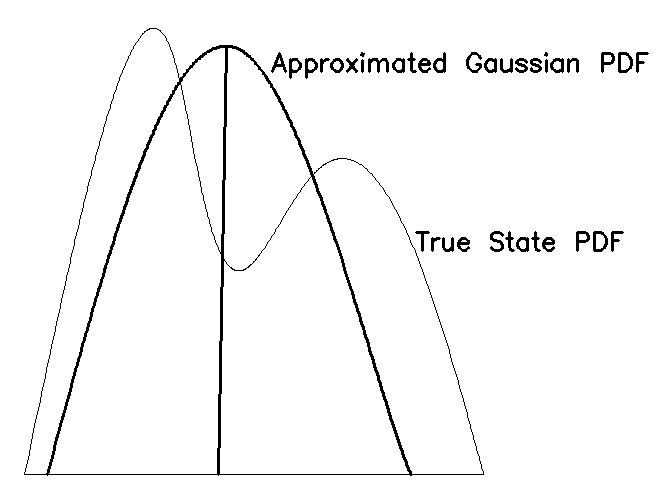
\includegraphics[width=0.35\textwidth]{approxgausspdf.jpg}
	\caption{First Approximations }
\end{figure}
\begin{figure}[h]
	\centering
		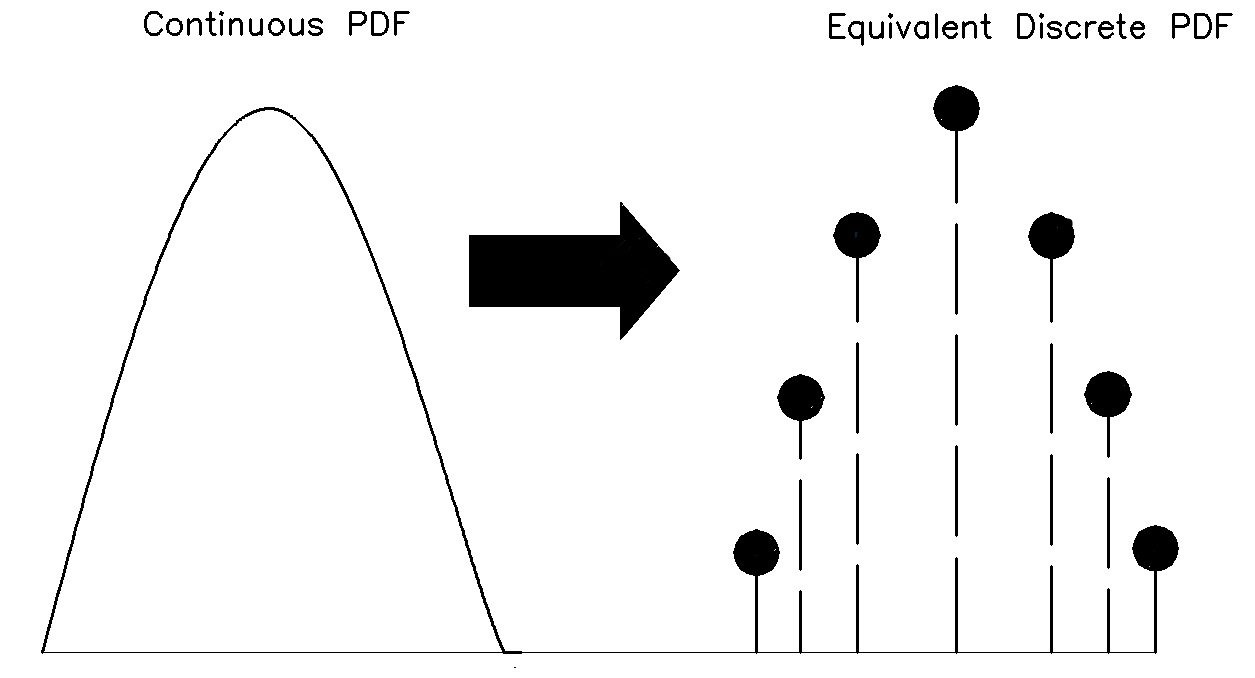
\includegraphics[width=0.4\textwidth]{conttodisc.jpg}
	\caption{Second Approximations}
\end{figure}
\end{comment}
%%%%%%%%%%%%%%%%%%%%%%
\begin{frame}
\begin{figure}[h]
	\centering
		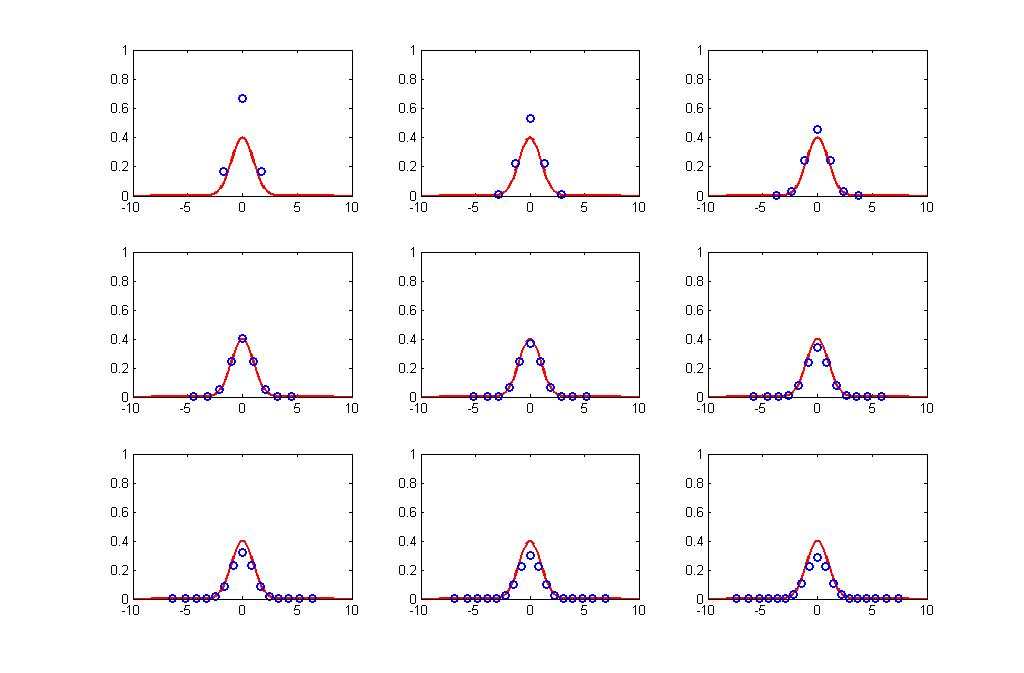
\includegraphics[width=1\textwidth]{contvsdisc.jpg}
	\caption{Guass hermite quadrature for 1D}
\end{figure}
\end{frame}
%%%%%%%%%%%%%%%%%%%%%%%%%
\begin{frame}
\frametitle{}
\begin{itemize}
\item In general for a N-Dimensional system, to integrate a polynomial of degree{\bf  $2m+1$ we need a total of $(m+1)^N$ quadrature points}. 
\item This is a {\bf very big number} for higher dimensional system and {\bf this is the basis of {\bf our motivation} to develop a method with reduced number of points}. 
\item Ideally one would like to capture all the {\bf infinite} moments of the PDF.
\item In practice this is difficult to achieve or might be computationally expensive. Thus often only the lower order moments are captured.This highly limits the type of funtions that can be integrated with good numerical accuracy.
\end{itemize}
\end{frame}

%%%%%%%%%%%%%%%%%%%%%%
\begin{frame}
\frametitle{Gauss Hermite Product rule}
\uncover<2->{The 1D Gauss Hermite rule can be extended to any dimension for an i.i.d set of random variable $(x_1,x_2,..x_N)^T$.}
\begin{align*}
\uncover<3->{E[f(x_1,x_2,...x_N)]}
\end{align*}
\begin{align*}
\uncover<4->{&=\int{\int{...\int{f(x_1,x_2,...x_N)N(x_1,x_2,...x_N,0|I)}}}dx_1dx_2...dx_N\\}
\uncover<5->{&=\int{\int{...[\int{f(x_1,x_2,...x_N)N(x_1,0|1)}}}dx_1]N(x_2,0|1)dx_2N(x_3,0|1)\\
&...N(x_N,0|1)dx_N}
\end{align*}
\begin{align*}
\uncover<6->{=\sum_{i_N=1}^n{w_N^{i_{N}}\sum_{i_{N-1}=1}^n{w_{N-1}^{i_{N-1}}...\sum_{i_2=1}^n{w_2^{i_2}\sum_{i_1=1}^n{w_1^{i_1}f(x_1^{i_1},x_2^{i_2},...x_N^{i_N})}}}}}
\end{align*}
\end{frame}
%%%%%%%%%%%%%%%%%%%%%%
\begin{frame}
\begin{figure}[h]
	\centering
		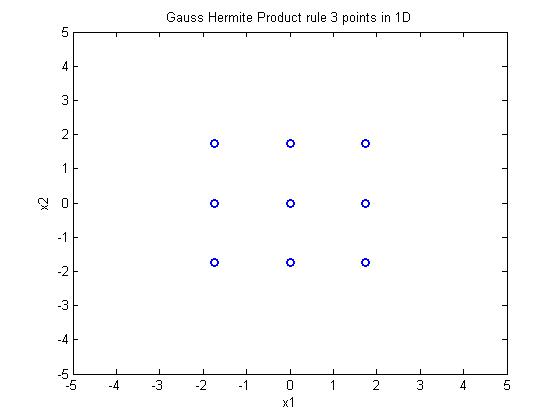
\includegraphics[width=0.5\textwidth]{eyegausshermite3points.jpg}
		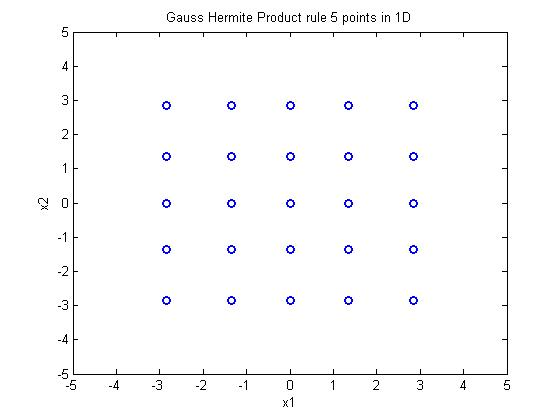
\includegraphics[width=0.5\textwidth]{eyegausshermite5points.jpg}
	\caption{Guass hermite product rule for 2D}
\end{figure}
\end{frame}
%%%%%%%%%%%%%%%%%%%%%%
\begin{frame}
\frametitle{Transformation of a Normal PDF with Arbitrary mean and Covariance into a Normal PDF with Zero Mean and Identity Covariance}
\begin{itemize}[<+->]
\item Any jointly distributed Normal PDF can be transformed into a Gaussian PDF of zero mean and identity covariance of same dimension. 
\item This way one could find the cubature points in the i.i.d space and then transform each point into the original jointly distributed space. 
\end{itemize}
\begin{align*}
\uncover<4->{	(x-\mu)^TP^{-1}(x-\mu)=(x-\mu)^TU^T\Sigma U(x-\mu)\\} 
\uncover<5->{	=(x-\mu)^TU^T\sqrt{\Sigma}\sqrt{\Sigma} U(x-\mu)} 
	\end{align*}
	\begin{align*}
	\uncover<6->{y=\sqrt{\Sigma}U(x-\mu)\\}
	\uncover<7->{(x-\mu)^TP^{-1}(x-\mu)=y^Ty} 
	\end{align*}
\end{frame}
%%%%%%%%%%%%%%%%%%%%%%
\begin{frame}
\begin{figure}[h]
	\centering
		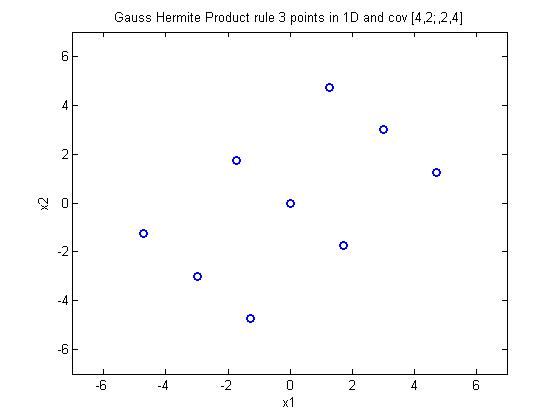
\includegraphics[width=0.5\textwidth]{eyegausshermite3pointsarbitcov.jpg}
		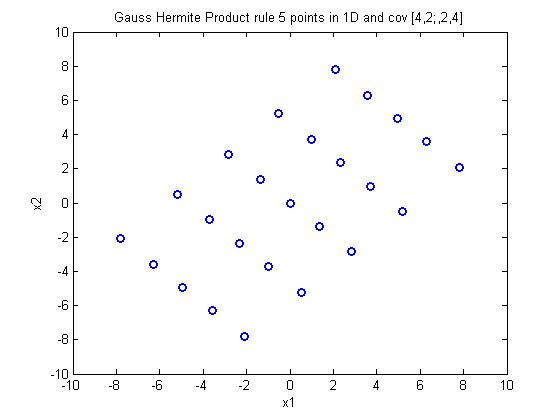
\includegraphics[width=0.5\textwidth]{eyegausshermite5pointsarbitcov.jpg}
	\caption{Guass hermite product rule for 2D for Cov $[4,2;2,4]$}
\end{figure}
\end{frame}
%%%%%%%%%%%%%%%%%%%%%
\begin{frame}
\frametitle{Evaluating the Cubature points}
To evalute the cubature points and weights of any PDF, the following procedure is followed 
\begin{itemize}[<+->]
\item Evaluate the{\bf  moments} of the continuous PDF
\item Assume the{\bf positions and weights} of each cubature point as variables
\item Equate the expressions of moment equations for the discrete system to the known moments of the continuous PDF
\item Solve these set of {\bf nonlinear moment constraint equations} 
\end{itemize}
\end{frame}
%%%%%%%%%%%%%%%%%%%%%%
\begin{frame}
\frametitle{Moment constraint equations  }
 The equivalent discrete moments are written interms of the assumed variables- {\bf positions and weights}
\uncover<2->{
\begin{table}
\caption{Equivalent Moments for 2D till order 4}
\label{moment_match}
\begin{center}
\begin{tabular}{|c|c||c|c|}
\hline
Continuous & Discrete & Continuous & Dicrete\\
\hline
$E[x]$ & $\sum_{i=1}^n{w_ix_i}$& $E[y]$ & $\sum_{i=1}^n{w_iy_i}$\\
\hline
$E[x^2]$ & $\sum_{i=1}^n{w_ix_i^2}$& $E[xy]$ & $\sum_{i=1}^n{w_ix_iy_i}$\\
\hline
$E[y^2]$ & $\sum_{i=1}^n{w_iy_i^2}$& $E[x^4]$ & $\sum_{i=1}^n{w_ix_i^2}$ \\
\hline
$E[y^4]$ & $\sum_{i=1}^n{w_iy_i^2}$& $E[x^3y]$ & $\sum_{i=1}^n{w_ix_i^3y_i}$\\
\hline
$E[y^3x]$ & $\sum_{i=1}^n{w_iy_i^3x_i}$ & $E[x^2y^2]$ & $\sum_{i=1}^n{w_ix_i^2y_i^2}$\\
\hline
\end{tabular}
\end{center}
\end{table}}
\uncover<3->{Table \ref{moment_match} gives the moment constraint equations that have to be solved for the {\bf weights $w_i$ and points $x_i$.}}

\end{frame}
%%%%%%%%%%%%%%%%%%%%%%
\begin{frame}
\frametitle{Moments of Continuous Normal PDF}
\begin{itemize}[<+->]
\item The higher order moments of a Normal PDF can be calculated from {\bf just the mean and Covariance.}
\item Particularly the Higher order raw moments just need the covariance matrix. 
\end{itemize}
\uncover<4->{The moments are given by the following theorem}
\uncover<5->{\begin{block}{Isserilis Theorem}
\begin{align*}
 E[x_1x_2x_3....x_{2n}]=\sum\prod{E[x_ix_j]}
 \end{align*} 
\end{block}}
\end{frame}
%%%%%%%%%%%%%%%%%%%%%%%%%%%%%%%%%%%
\begin{frame}
 for example the {\bf fourth moment} is
 \uncover<2->{\begin{equation*}
 E[x_1x_2x_3x_4]=E[x_1x_2]E[x_3x_4]+E[x_1x_3]E[x_4x_5]+E[x_1x_4]E[x_2x_3]
 \end{equation*}}
 \uncover<3->{And the {\bf sixth moment} is
 \begin{align*}
 E[x_1x_2x_3x_4x_5x_6]=
 \end{align*}
 \begin{align*}
 =&E[x_1x_2]E[x_3x_4]E[x_5x_6]    +E[x_1x_2]E[x_3x_5]E[x_4x_6]\\
 &+E[x_1x_2]E[x_3x_6]E[x_4x_5]    +E[x_1x_3]E[x_2x_4]E[x_5x_6]\\
 &+E[x_1x_3]E[x_2x_5]E[x_4x_6]		+E[x_1x_3]E[x_2x_6]E[x_4x_5]\\
 &+E[x_1x_4]E[x_2x_3]E[x_5x_6]		+E[x_1x_4]E[x_2x_5]E[x_3x_6]\\
 &+E[x_1x_4]E[x_2x_6]E[x_3x_5]    +E[x_1x_5]E[x_2x_3]E[x_4x_6]\\
 &+E[x_1x_5]E[x_2x_4]E[x_3x_6]		+E[x_1x_5]E[x_2x_6]E[x_3x_4]\\
 &+E[x_1x_6]E[x_2x_3]E[x_4x_5]		+E[x_1x_6]E[x_2x_4]E[x_3x_5]\\
 &+E[x_1x_6]E[x_2x_5]E[x_3x_4]
 \end{align*}}
\end{frame}
%%%%%%%%%%%%%%%%%%%%%%
\begin{frame}
\frametitle{Normal Distribution}
As the Normal PDF is symmetric, we would like to {\bf exploit this symmetry} in finding the cubature points. The points we like to seek have the following properties 
\begin{itemize}[<+->]
\item {\bf Fully symmetric} :- thus satisfying all odd order moments at no further cost
\item Weights {\bf sum up} to 1
\item All weights are to be {\bf positive}
\item As the points are symmetric, each point has an equivalent point located on the other side of the mean at the same distance.
\item These two points together lie on a line passing through the mean. We later name this line as  a particular {\bf 'axis'.} 
\item And these two points also have the same weight to balance each other
\end{itemize}
\end{frame}
%%%%%%%%%%%%%%%%%%%%%%
\begin{frame}
\frametitle{Terminology}
\uncover<2->{To proceed with the method we describe, the following {\bf terminology or definitions} that might be handy}
\begin{block}{Generator set}
\begin{itemize}[<+->]
\item This definition has been used quite a lot in literature to describe a set containing all permutations, including sign permutations of the elements in a set $\{u_1,u_2,u_3,...,u_r,0,0,0....,0\}$, where $u_1,u_2,...$ are real numbers.
\item for example the generator set $(1,1,0)$ is equivalent to $(1,1,0)$, $(1,0,1)$, $(0,1,1)$, $(-1,1,0)$, $(1,-1,0)$, $(-1,0,1)$, $(1,0,-1)$, $(0,-1,1)$, $(0,1,-1)$, $(0,-1,-1)$, $(-1,-1,0)$, $(-1,0,-1)$
\end{itemize} 
\end{block}
\uncover<5->{We introduce some new terminology with respect to the Identity Covariance Normal PDF of $N^{th}$-Dimension with zero mean, that will just aid our intuition }
\end{frame}
%%%%%%%%%%%%%%%%%%%%%%
\begin{frame}
\frametitle{The variables used}
\begin{itemize}[<+->]
\item Once the appropriate axis are chosen, the points are constrained to be on these axis such that a symmetric set of points that have the same weight are at equal distance from the origin.
\item The distance variables are $r_1$, $r_2$... measured from the origin to the appropriate set of points. 
\item The points at distance $r_1$ have weight $w_1$ and so on. 
\end{itemize}
\uncover<5->{
\begin{figure}[h]
	\centering
		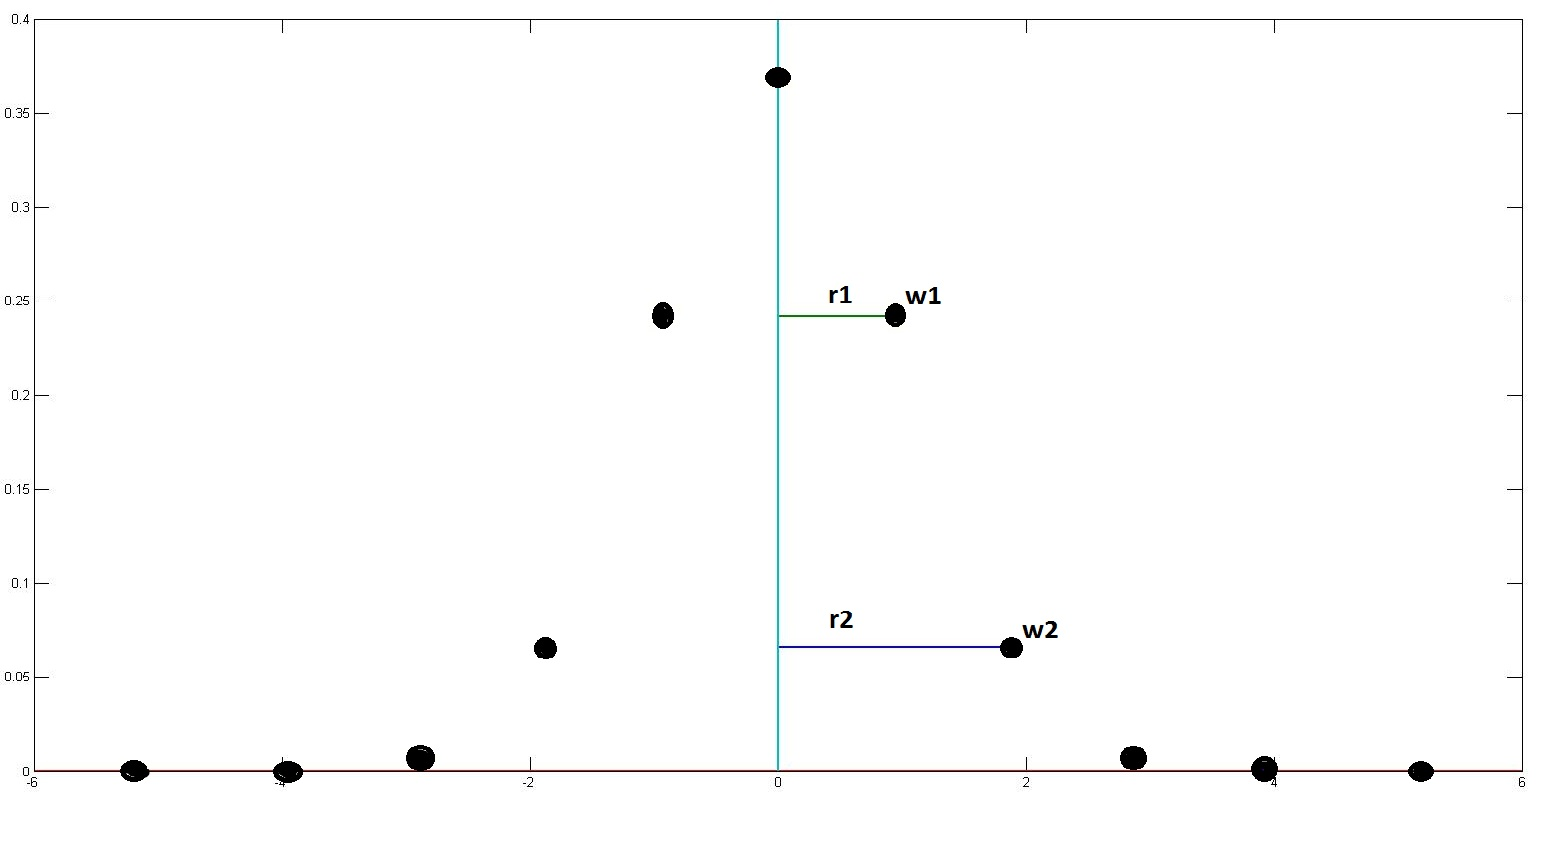
\includegraphics[width=0.5\textwidth]{1dgaussr1w1.jpg}
	\caption{distances and weights}
\end{figure}}
\end{frame}
%%%%%%%%%%%%%%%%%%%%%%
\begin{frame}
\begin{block}{Principle axis}
The axis formed from the generator set $\{1,0,0,...,0\}$. For example consider the 3D case for which the generator set is $\{(1,0,0)$, $(0,1,0)$, $(0,0,1)$, $(-1,0,0)$, $(0,-1,0)$, $(0,0,-1)\}$. The equivalent principle axis are just the orthogonal axis in 3D space $(1,0,0)$, $(0,1,0)$ and $(0,0,1)$. There are $2N$ points and N principle/orthogonal axis
\end{block}
\begin{figure}[h]
	\centering
		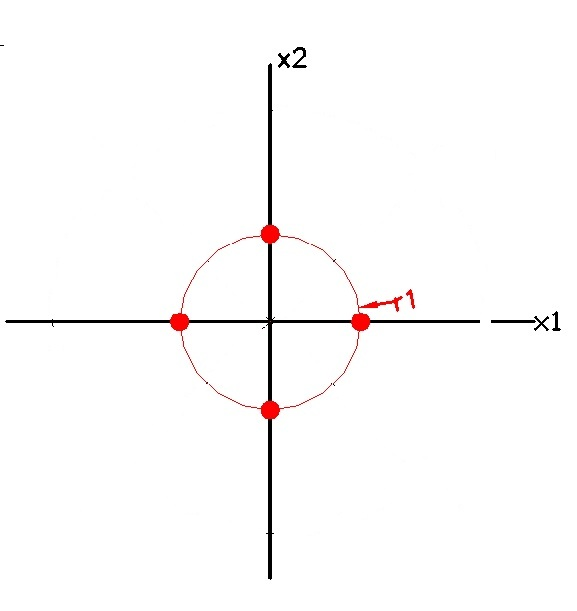
\includegraphics[width=0.3\textwidth]{2dprincipleaxis.jpg}
		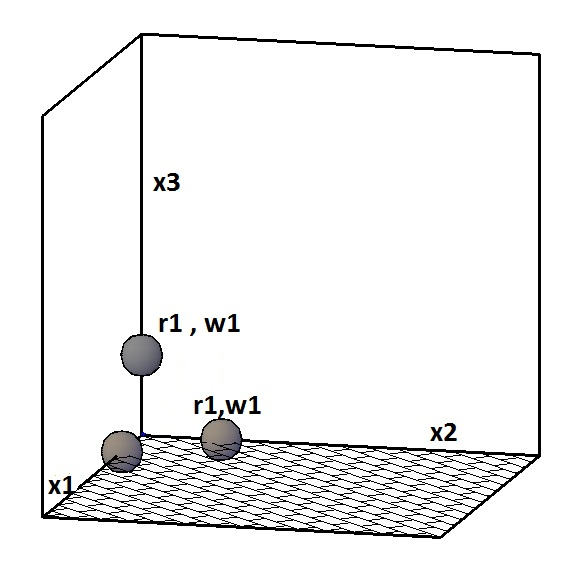
\includegraphics[width=0.3\textwidth]{3dprincipleaxis.jpg}
	\caption{distances and weights}
\end{figure}
\end{frame}
%%%%%%%%%%%%%%%%%%%%%%
\begin{frame}
\begin{block}{$M^{th}$-Conjugate axis}
\begin{itemize}[<+->]
\item For a Normal PDF of Nth Dimension, the axis that are formed from the generator set $\{1,1,1,...,1 \}$. 
\item For a 3D system the $3^{rd}$-conjugate axis are the lines that pass through the origin and the points from the generator set $(1,1,1)$, $(-1,1,1)$, $(1,-1,1)$, $(1,1,-1)$, $(-1,-1,1)$, $(1,-1,-1)$, $(-1,1,-1)$, $(-1,-1,-1)$. 
\item There are $2^N$ points $2^{(N-1)}$ axis. 
\item The $2^{nd}$- conjugate axis for a 3D system are the axis formed from the generator set $\{1,1,0\}$ 
\item The set of points $(1,1,0)$, $(1,0,1)$, $(0,1,1)$, $(-1,1,0)$, $(1,-1,0)$, $(-1,0,1)$, $(1,0,-1)$, $(0,-1,1)$, $(0,1,-1)$, $(0,-1,-1)$, $(-1,-1,0)$, $(-1,0,-1)$ 
\item There are $2N(N-1)$ points and $N(N-1)$ axis
\end{itemize}
\end{block}
\end{frame}
%%%%%%%%%%%%%%%%%%%%%%%%
\begin{frame}
\begin{figure}[h]
	\centering
	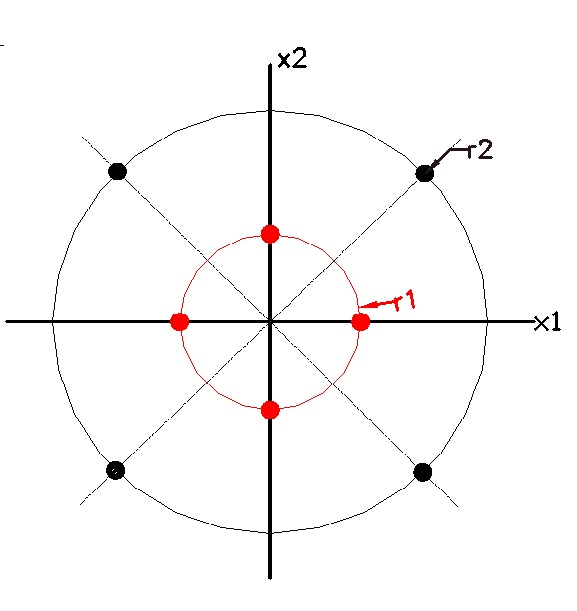
\includegraphics[width=0.25\textwidth]{2dconjaxis.jpg}
\end{figure}
\begin{figure}[h]
	\centering
		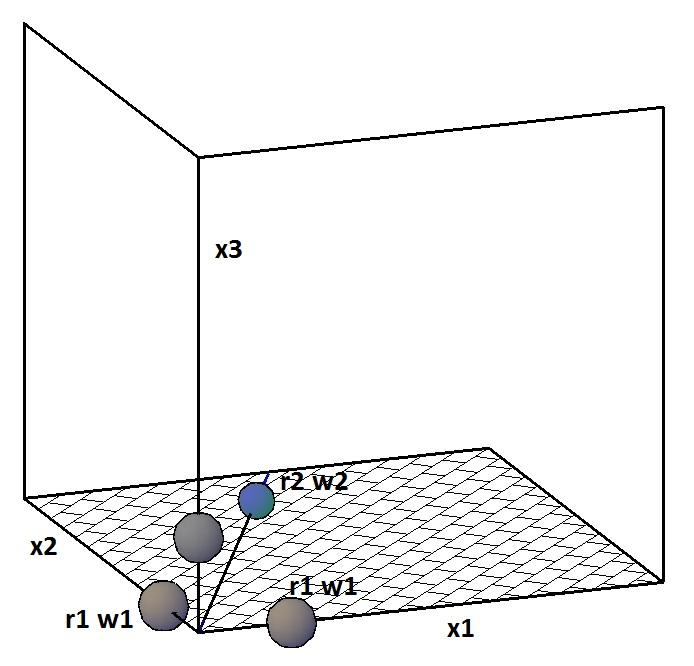
\includegraphics[width=0.4\textwidth]{3dnthconjaxis.jpg}
			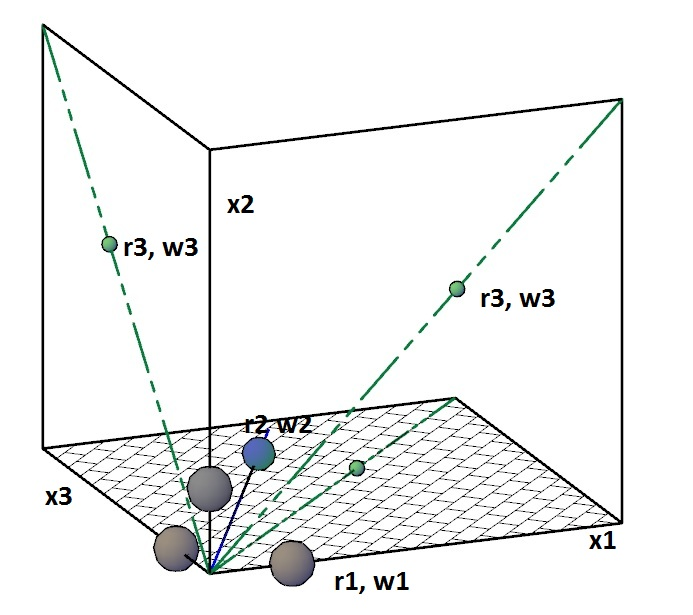
\includegraphics[width=0.4\textwidth]{3dnthconjand2ndconj.jpg}
	\caption{distances and weights}
\end{figure}
\end{frame}
%%%%%%%%%%%%%%%%%%%%%%
\begin{frame}
\begin{block}{$N^{th}$- Scaled Conjugate axis}
\begin{itemize}[<+->]
\item For a Normal PDF of Nth Dimension, the axis that are formed from the generator set $\{h,1,1,...,1 \}$. 
\item For a 3D system the $3^{rd}$-Scaled conjugate axis are the lines that pass through the origin and the points from the generator set $(h,1,1)$, $(-h,1,1)$, $(h,-1,1)$, $(h,1,-1)$, $(-h,-1,1)$, $(h,-1,-1)$, $(-h,1,-1)$, $(-h,-1,-1)$, $(1,h,1)$, $(-1,h,1)$, $(1,-h,1)$, $(1,h,-1)$, $(-1,-h,1)$, $(1,-h,-1)$, $(-1,h,-1)$, $(-1,-h,-1)$, $(h,1,1)$, $(-h,1,1)$, $(1,-1,h)$, $(1,1,-h)$, $(-1,-1,h)$, $(1,-1,-h)$, $(-1,1,-h)$, $(-1,-1,-h)$.
\item There are $N2^N$ points and $N2^{(N-1)}$ axis. 
\end{itemize}
\end{block}
\end{frame}
%%%%%%%%%%%%%%%%%%%%%%%%%%%
\begin{frame}
\begin{figure}[h]
	\centering
	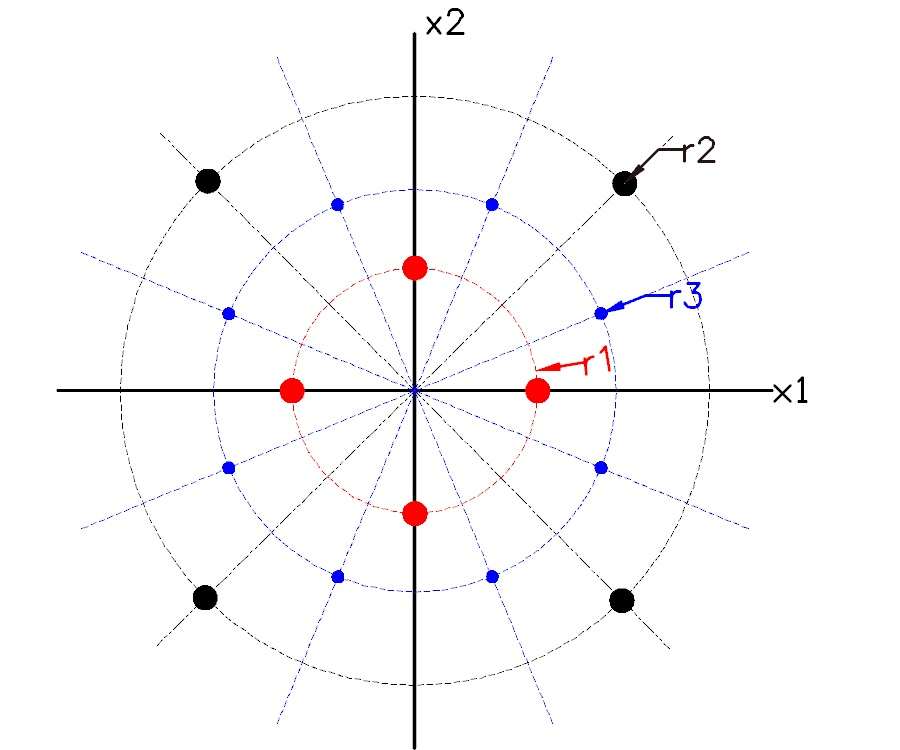
\includegraphics[width=0.25\textwidth]{2dhscaledaxis.jpg}
\end{figure}

\begin{figure}[h]
	\centering
		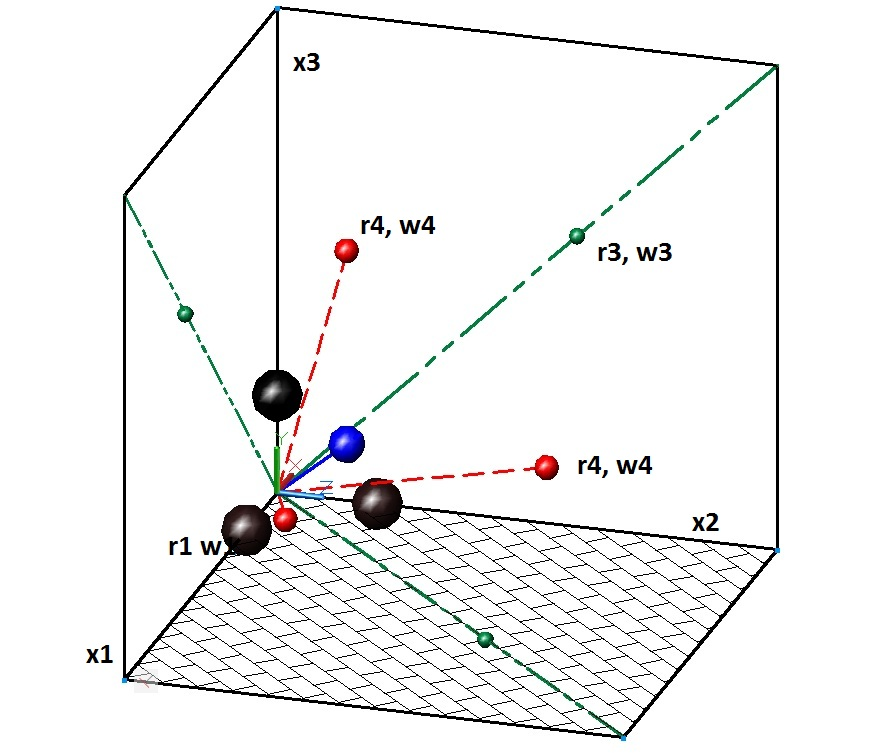
\includegraphics[width=0.4\textwidth]{3dhscaledaxis.jpg}
			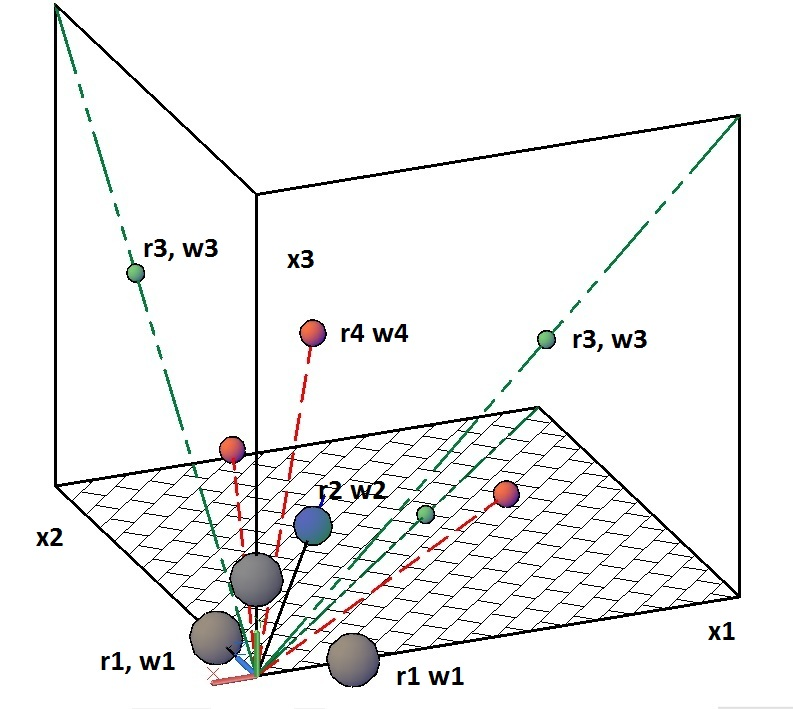
\includegraphics[width=0.4\textwidth]{3dhscaledaxis2.jpg}
	\caption{distances and weights}
\end{figure}
\end{frame}

%%%%%%%%%%%%%%%%%%%%%%
\begin{frame}
\frametitle{Cubature points constrained to the principle axis to satisfy the $2^{nd}$ order moments}
\uncover<2->{For an i.i.d random variables $(X_1,X_2,...,X_N)$ the N-Dimensional normal PDF has Identity covariance and zero mean. The {\bf first four moments} of this continuous PDF are}
\begin{align*}
\uncover<3->{E[X_i^2]&=1\\}
\uncover<4->{E[X_iX_j]&=0\\}
\uncover<5->{E[X_i^4]&=3\\}
\uncover<6->{E[X_i^3X_j]&=0\\}
\uncover<7->{E[X_i^2X_j^2]&=1\\}
\uncover<8->{E[X_i^2X_jX_k]&=0\\}
\uncover<9->{E[X_iX_jX_kX_l]&=0}
\end{align*}
\uncover<10->{Where $\{i,j,k,l\}\in\{1,2,3,...,N\}$ $\&$ $i \neq j \neq k \neq l$.}
\end{frame}
%%%%%%%%%%%%%%%%%%%%%%
\begin{frame}
\begin{itemize}[<+->]
\item Consider a fully symmetric set of cubature points that lie on the principle axis at a distance of $r_1$ from the origin and have weight of $w_1$. 
\item The moments that have any odd powers for the random varable in the set of moments is are already satisfied due to{\bf  symmetry of cubature points.}
\item Only the moments with {\bf all even powers} have to be satisfied
\end{itemize}
\begin{align*}
\uncover<5->{E[X_i^2]&=1\\}
\uncover<6->{E[X_i^4]&=3\\}
\uncover<7->{E[X_i^2X_j^2]&=1}
\end{align*}
\end{frame}
%%%%%%%%%%%%%%%%%%%%%%%%%%%%%%%%%%%%%%%%%%
\begin{frame}
\begin{figure}[h]
	\centering
		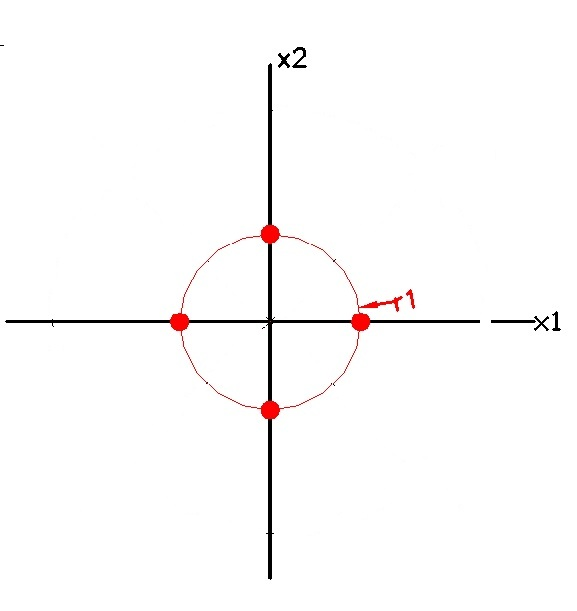
\includegraphics[width=0.3\textwidth]{2dprincipleaxis.jpg}
	\caption{distances and weights}
\end{figure}
\uncover<2->{For example consider the 2D system. The points on these axis when enumerated as a list is $(r1,0)$, $(0,r1)$, $(-r1,0)$, $(0,-r1)$. The equivalent discrete moments are}
\begin{align*} 
\uncover<3->{2r_1^2w_1&=1\\}
\uncover<4->{2r_1^4w_1&=3\\}
\uncover<5->{0\neq1}
\end{align*}
\end{frame}
%%%%%%%%%%%%%%%%%%%%%%%%%%%%%%%%%%%%%%%%%%%%%
\begin{frame}
\uncover<2->{This set of equations are infact the same for any dimension.The central weight is calculated as}
\begin{equation}
\uncover<3->{w_0=1-2Nw_1}
\end{equation}
\uncover<4->{One of the $4^{th}$ order cross moment {\bf cannot be satisfied} by selecting such points on the principle axis.}\newline
\uncover<5->{ In general {\bf no cross moment} of any order can be satisfied by the points just on the {\bf principle axis.} }
\begin{equation}
\uncover<6->{E[X_i^2X_j^2]\neq1}
\end{equation}
\uncover<7->{The 4th moment is also evaluted here just to compare different filters such as UKF and CKF in terms of the {\bf 4th order moment error}.}
\end{frame}
%%%%%%%%%%%%%%%%%%%%%%%%%%%%%%%%%%%%%%%%%%
\begin{frame}
\frametitle{The $2N+1$ Unscented Transform Method }
\begin{itemize}[<+->]
\item The $2N+1$ sigma points for the unscented Transform are chosen such that 1 point is the origin and $2N$ points of equal weight are constrained to lie on the principle axis. 
\item The distance of each point on the principle axis is chosen such that the second order moments are satisfied. 
\item A tuning parameter $\kappa$ is introduced such that one of the 4th moment can be tuned. 
\item This works well for systems till dimension 3 after which the central weight becomes negative. 
\item The present framework is shown to {\bf be inline} with the $2n+1$ Unscented sigma points by working our way backwards.
\end{itemize}
\end{frame}
%%%%%%%%%%%%%%%%%%%%%%%%%%%%%%%%%%%%%%%%%%%%%
\begin{frame}
 The suggested points by the authors of UT paper are
\begin{align*}
\uncover<2->{x_0&=\mu \quad &w_0=\frac{\kappa}{(N+\kappa)}\\}
\uncover<3->{x_i&=\mu+(sqrt{(N+\kappa)P})_i\quad  &w_i=\frac{1}{2(N+\kappa)}\\}
\uncover<4->{x_{i+N}&=\mu-(sqrt{(N+\kappa)P})_i\quad 	 &w_{i+N}=\frac{1}{2(N+\kappa)}}
\end{align*}
\uncover<5->{An {\bf elegant selection for $r_1$} is chosen and then rest of the variables are solved in terms of this selction}
\begin{align*}
\uncover<6->{r_1&=\sqrt{N+\kappa}\\}
\uncover<7->{w_1&=\frac{1}{2(N+\kappa)}\\}
\uncover<8->{w_0&=1-2Nw_1=\frac{\kappa}{(N+\kappa)}\\}
\uncover<9->{2r_1^4w_1 & \equiv N+\kappa=3}
\end{align*}
\end{frame}
%%%%%%%%%%%%%%%%%%%%%%%%%%%%%%%%%%%%%%%%%%%%%
\begin{frame}
\frametitle{The $2N$ Cubature Kalman Filter}
\begin{itemize}[<+->]
\item The authors of CKF provide a very mathematically rigourous and elegant way of of finding the second moment equivalent $2N$ cubature points that can again accurately integrate polynomials of degree 3 or less.
\item Spherical-radial coordinates are employed rather than cartesian coordinates to find these $2N$ symmetric cubature points on the principle axis. 
\item Contrary to the $2N+1$ Unscented transform sigma points, they only have $2N$ cubature  points on the principle axis and no point on the mean. 
\end{itemize}
\end{frame}
%%%%%%%%%%%%%%%%%%%%%%%%%%%%%%%%%%%%%%%%%%%%%
\begin{frame}
\begin{itemize}[<+->]
\item This is equivalent to {\bf setting $\kappa=0$} in the Unscented transform sigma points thus making the central weight $w_0$ 0. 
\item An alternate derivation  to the one given in their paper is provided which is less rigourous but {\bf more intuitive} using the present frame work.
\end{itemize}
\uncover<4->{As there is no point at the mean, the central weight can be taken 0. }
\begin{align*}
\uncover<5->{0&=1-2Nw_1\\}
\uncover<6->{w_1&=\frac{1}{2N}\\}
\uncover<7->{r_1&=\sqrt{N}}
\end{align*}
\end{frame}
%%%%%%%%%%%%%%%%%%%%%%%%%%%%%%%%%%%%%%%%%%%%%%%
\begin{frame}
\frametitle{Comparison of UT and CKF cubature points using the error in the 4th moment}
\begin{itemize}[<+->]
\item The authors of CKF claim that their method is superior to UKF. They outrightly criticize that UT has no mathematical basis.
\item Infact the UT can {\bf capture one of the 4th order moment exactly} but the CKF has an error in all the fourth order moments.
\item This is also illustrated by examples later on in the results section. 
\end{itemize}
\uncover<5->{Absolute error in fourth moment for UT}
\begin{equation}
\uncover<6->{|3-(N+\kappa)|}
\end{equation}
\uncover<7->{Absolute error in fourth moment for CKF}
\begin{equation}
\uncover<8->{|2N^2\frac{1}{2N}-3|\equiv |N-3|}
\end{equation}
\end{frame}
%%%%%%%%%%%%%%%%%%%%%%%%%%%%%%%%%%%%
\begin{frame}
\frametitle{Cubature points that are 4th order equivalent}
\begin{itemize}[<+->]
\item The authors of UT suggest a method to capture the fourth order moments
\item But this method suffers the same problem of having a {\bf negative weight above dimension 4}.
\item The authors suggest to constrain 1 set of points on the principle axis and another set on the $2^{nd}$-conjugate axis
\item A formal derivation in terms of the present framework is shown 
\end{itemize}
\begin{align*}
\uncover<6->{2r_1^2w_1+4(N-1)r_2^2w_2=1\\}
\uncover<7->{2r_1^4w_1+4(N-1)r_2^4w_2=3\\}
\uncover<8->{4r_2^4w_1=1\\}
\uncover<9->{1-2Nw_1-2N(N-1)w_2=w_0}
\end{align*}
\end{frame}
%%%%%%%%%%%%%%%%%%%%%%%%%%%%%%%%%%%%
\begin{frame}
\frametitle{ }
The simplified set of equations are got by first solving for $w_1$ and $w_2$ and then substituting them in the first equation
\begin{align*}
\uncover<2->{w_2=\frac{1}{4r_2^4}\\}
\uncover<3->{w_1=\frac{4-N}{2r_1^4}}
\end{align*}
\uncover<4->{Substituting these weights into the first constraint equation we have only one cosntraint equation}
\begin{equation*}
\uncover<5->{r_1^2r_2^2=r_1^2(N-1)+r_2^2(4-N)}
\end{equation*}
\uncover<6->{Even though we solve for $r_1$ and $r_2$ we always have a negative/zero weight for $N>3$ }
\end{frame}
%%%%%%%%%%%%%%%%%%%%%%%%%%%%%%%%%%%%
\begin{frame}
\frametitle{The Conjugate Unscented Transform Method  to capture all the 4th moment}

\begin{itemize}[<+->]
\item The first set of points are chosen on the principle axis at a distance of $r_1$ and weight $w_1$ each.
\item The second set of points are chosen on the Nth-Conjugate axis at a distance of $r_2$ and each have a weight of $w_2$.
\end{itemize}
\uncover<4->{Forming the moment constraint equations along with the central weight}
\begin{align*}
\uncover<5->{2r_1^2w_1+2^Nr_2^2w_2&=1\\}
\uncover<6->{2r_1^4w_1+2^Nr_2^4w_2&=3\\}
\uncover<7->{2^Nr_2^4w_2&=1\\}
\uncover<8->{1-2Nw_1-2^Nw_2&=w_0}
\end{align*}
\end{frame}
%%%%%%%%%%%%%%%%%%%%%%%%%%%%%%%%%%%%
\begin{frame}
\begin{figure}[h]
	\centering
	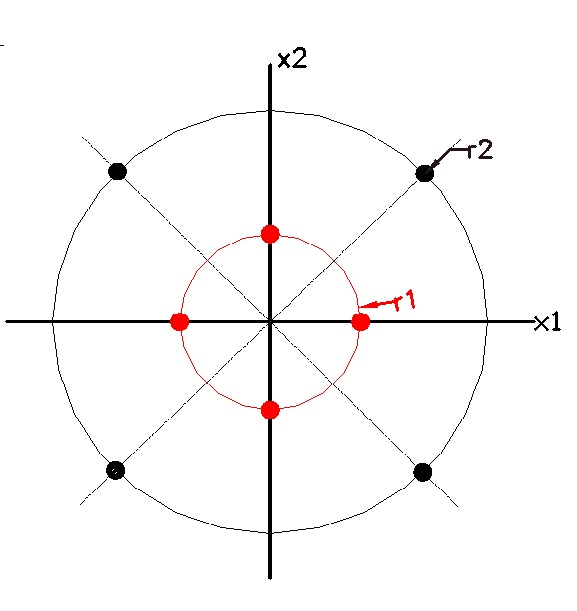
\includegraphics[width=0.25\textwidth]{2dconjaxis.jpg}
\end{figure}
\begin{figure}[h]
	\centering
	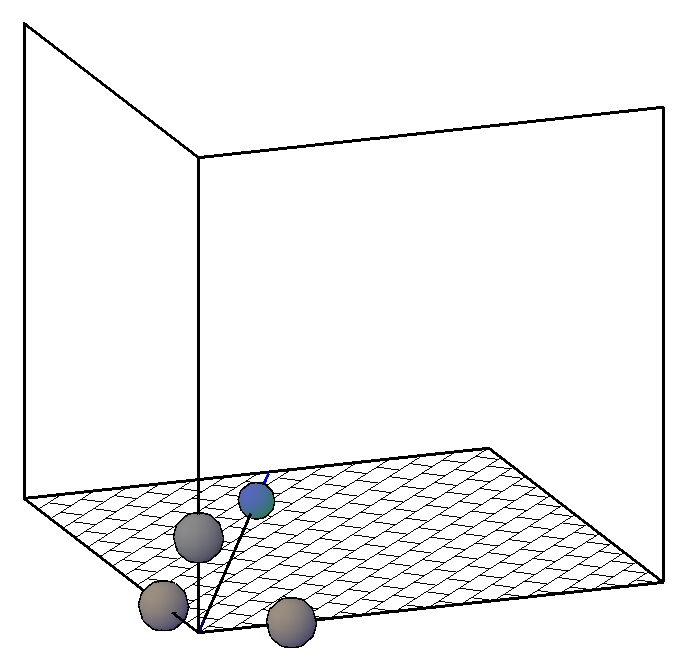
\includegraphics[width=0.4\textwidth]{4thmoment3d1.jpg}
	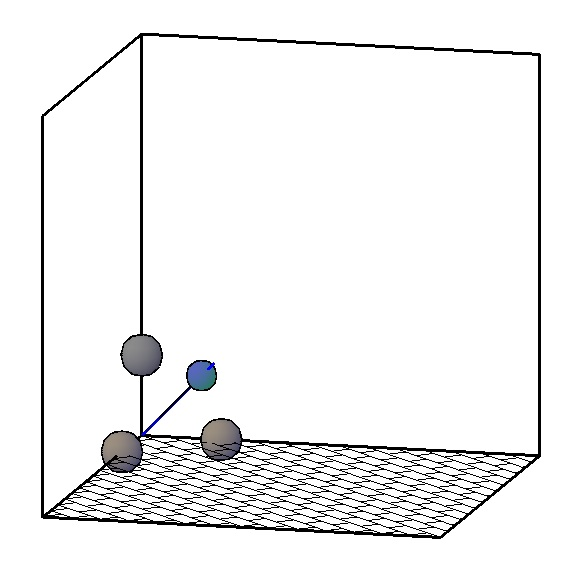
\includegraphics[width=0.4\textwidth]{4thmoment3d3.jpg}
	\caption{distances and weights}
\end{figure}
\end{frame}
%%%%%%%%%%%%%%%%%%%%%%%%%%%%%%%%%%
\begin{frame}
These set of equations can be {\bf solved analytically} in the following 2 schemes because there is no constraint on $w_0$ except that it should be positive\newline
\uncover<2->{{\bf Solution 1}}\newline
\uncover<3->{The $w_0$ is solved for by minimizing the square of error in sixth moment}
\begin{equation*}
\uncover<4->{Min \quad (2r_1^6w_1+2^Nr_2^6w_2-15)^2}
\end{equation*}
\uncover<5->{This is applied for dimensions 1 and 2}
\uncover<6->{
\begin{table}
\caption{Optimization Solution for $N=1$ and $N=2$ }
\label{optsoln12}
\begin{center}
\begin{tabular}{|c||c|c|}
\hline
Variable & $N=1$ & $N=2$\\
\hline
$r_1$ & $1.4861736616297834 $  &  $2.6060099476935847 $  \\
\hline
$r_2$ & $3.2530871022700643 $  &  $1.190556300661233 $  \\
\hline
$w_0$ & $0.5811010092660772 $  &  $0.41553535186548973 $  \\
\hline
$w_1$ & $0.20498484723245053 $  &  $0.021681819434216532 $  \\
\hline
$w_2$ & $0.00446464813451093 $  &  $0.12443434259941118 $  \\
\hline
\end{tabular}
\end{center}
\end{table}}
\end{frame}
%%%%%%%%%%%%%%%%%%%%%%%%%%%%%%%%%%
\begin{frame}
{\bf Solution 2}
\uncover<2->{For dimension greater than 2, the central weight is eliminated thus {\bf reducing 1 point}.}
\uncover<3->{For $N>2$}
\begin{align*}
\uncover<4->{w_0=0\\}
\uncover<5->{r1=\sqrt{\frac{N+2}{2}}\\}
\uncover<6->{r2=\sqrt{\frac{N+2}{N-2}}\\}
\uncover<7->{w_1=\frac{1}{r_1^4}=\frac{4}{(N+2)^2}\\}
\uncover<8->{w_2=\frac{1}{2^Nr_2^4}=\frac{(N-2)^2}{2^N(N+2)^2}}
\end{align*}
\end{frame}
%%%%%%%%%%%%%%%%%%%%%%%%%%%%%%%%%%%%
\begin{frame}
\frametitle{ }
{\bf Results of integration compared to Gauss Hermite integration for 3D system}\newline
The total number of cubature points involved in this method to capture all the moments till 4th order is{\bf  $2N+2^N$}
\[
 P = \begin{bmatrix}
       4 & 2 & 1    \\
       2 & 9 & 1     \\
       1 & 1 & 16
     \end{bmatrix}
\]
\begin{align*}
F&=x_1^4+x_2^4+x_3^4+x_1^3x_2+x_1^2x_2^2+\\
 &+x_3^2x_2^2+x_1^2x_3^2+x_1^3x_3+x_2^3x_3+x_3^3x_2
\end{align*}
\end{frame}
%%%%%%%%%%%%%%%%%%%%%%%
\begin{frame}
\tiny
\begin{center}
  \begin{tabular}{ | l | l | l | l | l | }
    \hline
       No. of pts 					& $2^3=$ 8 							& $3^3=$ 27 			  & $4^3=$ 64			 & Analytical       \\ \hline 
      GH          					&   1056.95571  			  & 1797.99999      & 1798.00     	 &   1798.00           \\ \hline
\% error wrt Truth       	  &   41.2149211    			&  4.299e-013  	  	& 3.0350e-013   &   0         \\ 
      \hline
  \end{tabular}
\end{center} 
\uncover<2->{
\begin{center}
\normalsize
  \begin{tabular}{ | l | l | l | l | l | }
    \hline
                  					&   No. of pts			& Integration result 			  & \% error			 \\ \hline 
      CUT4          					&   15       			  & 1797.999999         & 6.3552080e-010   \\
      \hline
  \end{tabular}
\end{center}}
\end{frame}
%%%%%%%%%%%%%%%%%%%%%%%%%%%%%%%%%%%%
\begin{frame}
\frametitle{ }
{\bf Results of integration compared to Gauss Hermite integration for 8D system}\newline
The total number of cubature points involved in this method to capture all the moments till 4th order is $2N+2^N$
\begin{equation}
P=10I_{8x8}
\end{equation}
\begin{equation*}
F=x_1^4+x_8^2*x_2^2+x_3^2+x_4^2*x_5^2
\end{equation*}
\end{frame}
%%%%%%%%%%%%%%%%%%%%%%%
\begin{frame}
\tiny
\begin{center}
  \begin{tabular}{ | l | l | l | l | l | }
    \hline
  No. of pts 					      & $2^8=$ 8 					& $3^8=$ 6561 		  & $4^8=$ 65536			 & Analytical       \\ \hline 
      GH          					&   256             & 614               & 614     	         &   614           \\ \hline
   \% error             	  &   32.573   	      & 5.18441605e-013  	& 6.591614e-012      &   0         \\ 
      \hline
  \end{tabular}
\end{center} 
\uncover<2->{
\begin{center}
\normalsize
  \begin{tabular}{ | l | l | l | l | l | }
    \hline
                  					&   No. of pts			& Integration result 			  & \% error 			 \\ \hline 
     CUT4          					&   273       			& 614                       &  1.0368832104e-012   \\
      \hline
  \end{tabular}
\end{center}}
\end{frame}
%%%%%%%%%%%%%%%%%%%%%%%%%%%%%%%%%%%%
\begin{frame}
\frametitle{ }
{\bf Cubature points that are $6^{th}$ order equivalent}\newline
\begin{itemize}[<+->]
\item We {\bf attempt} to capture all the $6^{th}$ order moments till 6D
\item In addition to the axis chosen for the fourth moment one additional set of axis is considered
\item 1 point on the mean, first set of points on the principle axis at distance $r_1$ and each weight $w_1$.
\item Second set on the Nth-Conjugate axis with distance $r_2$ and weight $w_2$.
\item Third set of axis are chosen on the 2nd conjugate axis with points at distance $r_3$ and weight $w_3$
\end{itemize}
\end{frame}
%%%%%%%%%%%%%%%%%%%%%%%%%%%%%%%%%%%%%
\begin{frame}
\begin{figure}[h]
	\centering
		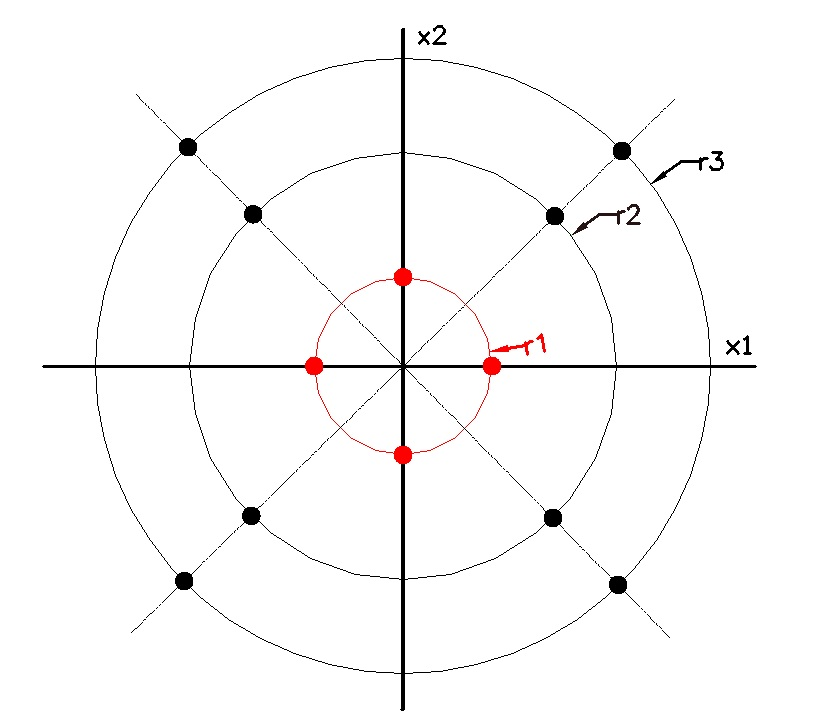
\includegraphics[width=0.25\textwidth]{6thmoment2d1.jpg}
\end{figure}

\begin{figure}[h]
	\centering
		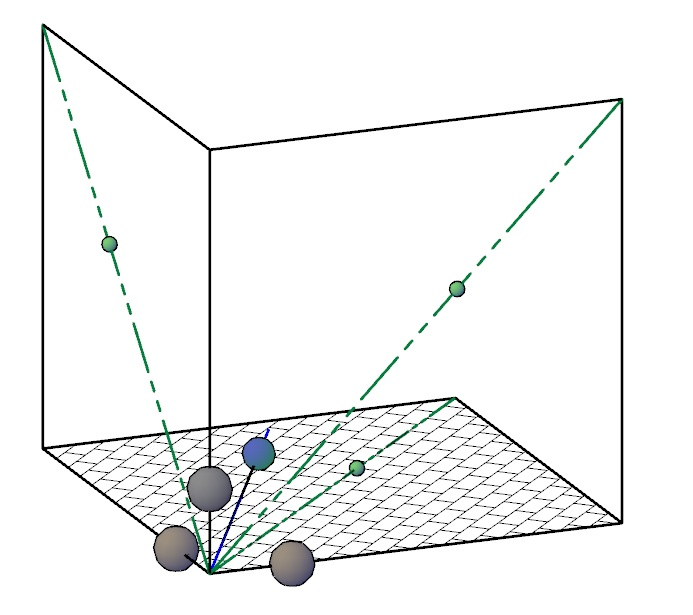
\includegraphics[width=0.4\textwidth]{3d6thmom.jpg}
		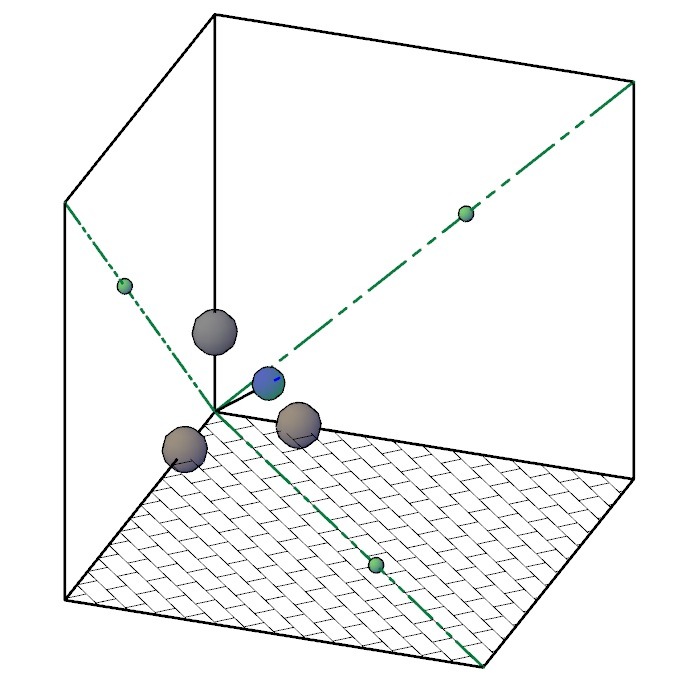
\includegraphics[width=0.4\textwidth]{3d6thmom2.jpg}
	\caption{distances and weights}
\end{figure}

\end{frame}
%%%%%%%%%%%%%%%%%%%%%%%%%%%%%%%%%%%%
\begin{frame}
\frametitle{Moments till 6th order}
\begin{align*}
\uncover<2->{E[X_i^2]&=1 \quad &E[X_iX_j]=0\\}
\uncover<3->{E[X_i^4]&=3 \quad &E[X_i^3X_j]=0\\}
\uncover<4->{E[X_i^2X_j^2]&=1 \quad &E[X_i^2X_jX_k]=0\\}
\uncover<5->{E[X_iX_jX_kX_l]&=0 \quad &E[X_i^6]=15\\}
\uncover<6->{E[X_i^5X_j]&=0 \quad &E[X_i^4X_j^2]=3\\}
\uncover<7->{E[X_i^4X_jX_k]&=0 \quad &E[X_i^3X_j^3]=0\\}
\uncover<8->{E[X_i^3X_j^2X_k]&=0 \quad &E[X_i^3X_j^2]=0\\}
\uncover<9->{E[X_i^2X_j^2X_k^2]&=1 \quad &E[X_iX_jX_kX_lX_mX_n]=0}
\end{align*}
\end{frame}
%%%%%%%%%%%%%%%%%%%%%%%%%%%%%%%%%%%%
\begin{frame}
\frametitle{Moment constraint equations till order 6 }
\begin{align*}
\uncover<2->{2r_1^2w_1+2^Nr_2^2w_2+4(N-1)r_3^2w_3=1\\}
\uncover<3->{2r_1^4w_1+2^Nr_2^4w_2+4(N-1)r_3^4w_3=3\\}
\uncover<4->{2^Nr_2^4w_2+4r_3^4=1\\}
\uncover<5->{2r_1^6w_1+2^Nr_2^6w_2+4(N-1)r_3^6w_3=15\\}
\uncover<6->{2^Nr_2^6w_2+4r_3^6=3\\}
\uncover<7->{2^Nr_2^6w_2=1}
\end{align*}
\end{frame}
%%%%%%%%%%%%%%%%%%%%%%%%%%%%%%%%%%%%
\begin{frame}
\frametitle{Solution to the system }
\uncover<2->{Procedure followed}
\begin{itemize}[<+->]
\item These nonlinear equations are in a way linear with respect to the weights
\item The last 3 equations can be solved for $w_1$, $w_2$ and $w_3$ symbolically in terms of the other variables $r_1$, $r_2$ and $r_3$ 
\item Substituting these into the first 3 equations the overall order of the system is reduced.
\end{itemize}
\begin{align*}
\uncover<6->{w_1&=\frac{8-N}{r_1^6}\\}
\uncover<7->{w_2&=\frac{1}{2^Nr_2^6}\\}
\uncover<8->{w_3&=\frac{1}{2r_3^6}}
\end{align*}
\end{frame}
%%%%%%%%%%%%%%%%%%%%%%%%%%%%%%%%%%%
\begin{frame}
\frametitle{ }
{\bf Results of integration compared to Gauss Hermite integration for 4D system}\newline
The total number of cubature points involved in this method to capture all the moments till 6th order is $2N^2+2^N+1$
\[
 P = \begin{bmatrix}
       4 & 1 & 2  & 1   \\
       1 & 9 & 2  & 3   \\
       2 & 2 & 16 & 4  \\
       1 & 3 & 4 & 25  
     \end{bmatrix}
\]
\begin{align*}
F&=x_1^6+x_2^6+x_3^6+x_4^6+x_1^4+x_2^4+x_3^4+x_4^4+x_1^2x_2^2x_3^2+\\
&+x_1^3x_3+x_1^2x_2^4+x_3^4x_2^2+x_1^2x_3^4+x_1^3x_3+x_2^3x_3+x_3^3x_2
\end{align*}
\end{frame}
%%%%%%%%%%%%%%%%%%%%%%%%%%%%%%%%%%%%%%%%%%
\begin{frame}
\tiny
\begin{center}
\tiny
  \begin{tabular}{ | l | l | l | l | l | l | }
    \hline
 No. of pts   & $2^4=$ 16    & $3^4=$ 81 			& $4^4=$ 256		 & $5^4=$ 64 	  	      &   Analytical \\   \hline 
   GH        &   84462.6354  & 293311.8446    & 375417.9999    & 375417.9999          &   375417.9999  \\ \hline
\% error        	  &   77.5017    		&  21.8705  	  	& 9.0702e-012   & 8.9152e-012 &   0     \\        \hline 
  \end{tabular}
\end{center} 
\uncover<2->{
\begin{center}
\normalsize
  \begin{tabular}{ | l | l | l | l | l | }
    \hline
                  					&   No. of pts			& Integration result 			  & \% error 			 \\ \hline 
      CUT6         					&   49       			  & 3.7541800e+005            & 8.062475e-013   \\
      \hline
  \end{tabular}
\end{center}}
\end{frame}
%%%%%%%%%%%%%%%%%%%%%%%%%%%%%%%%%%%%%
\begin{frame}
\frametitle{ }
{\bf Results of integration compared to Gauss Hermite integration for 6D system}\newline
The total number of cubature points involved in this method to capture all the moments till 6th order is $2N^2+2^N+1$
\begin{equation}
P=10I_{6x6}
\end{equation}
\begin{equation*}
F=x_1^6+x_1^2x_2^2x_3^2+x_1^4x_6^2+x_5^4+x_3^2x_4^2
\end{equation*}
\end{frame}
%%%%%%%%%%%%%%%%%%%%%%%%%%%%%%%%%%%%%%%%%%
\begin{frame}
\tiny
\begin{center}
\tiny
  \begin{tabular}{ | l | l | l | l | l | l | }
    \hline
 No. of pts   & $2^6=$ 64      & $3^6=$ 729 			& $4^6=$ 4096		 & $5^6=$ 15625 	  	 &   Analytical \\   \hline 
   GH         & 6.035000e+003  & 1.943500e+004    & 2.543500e+004  & 2.543500e+004       &   2.5434999e+004  \\ \hline
\% error      &   76.2728  		 &  23.589 	  	    & 1.5633e-011    & 1.58906e-011        &   0     \\        \hline 
  \end{tabular}
\end{center} 
\uncover<2->{
\begin{center}
\normalsize
  \begin{tabular}{ | l | l | l | l | l | }
    \hline
                  					&   No. of pts			& Integration result 			  & \% error 			 \\ \hline 
      CUT6         					&   137       			& 2.543500e+004             & 3.4583111e-008   \\
      \hline
  \end{tabular}
\end{center}}
\end{frame}
%%%%%%%%%%%%%%%%%%%%%%%%%%%%%%%%%%%%%
\begin{frame}
\frametitle{Cubature points to capture ALL the 8th order moments}
\begin{itemize}[<+->]
\item All the axis used before were not able to capture all the 8th order moments
\item Only points that lie in the full N-D space enter the 8th order moments.
\item I was only able to capture the moments till 6th dimension.
\item Due to the complex nature of the equation I was not able to find a trend in the set of equations to generalize it.
\item I have only done this  case by case till 6th-DImension. 
\item But in all cases I have selected the {\bf SAME} set of axis
\end{itemize}
\end{frame}
%%%%%%%%%%%%%%%%%%%%%%%%%%%%%%%%
\begin{frame}
\begin{itemize}[<+->]
\item 1 point on the mean
\item A set of points on the principle axis
\item A set of points on the Nth-conjugate axis
\item A set of points on the 2nd-conjugate axis
\item A set of points on the Nth- Scaled conjugate axis
\item The scaling parameter h has to appropriately chosen
\end{itemize}
\uncover<8->{
\begin{figure}[h]
	\centering
		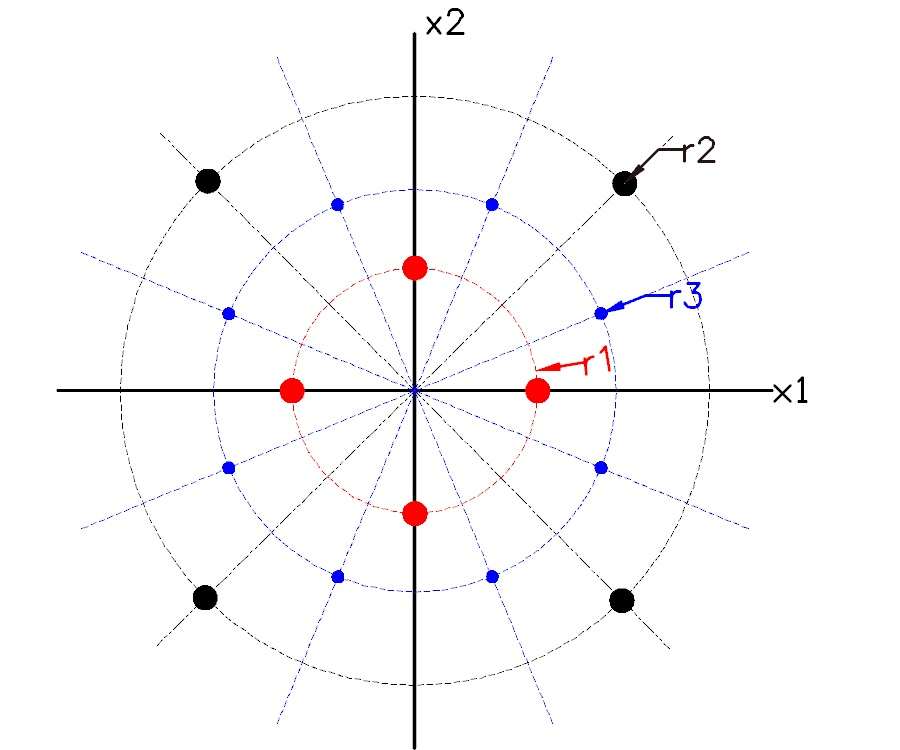
\includegraphics[width=0.3\textwidth]{2dhscaledaxis.jpg}
		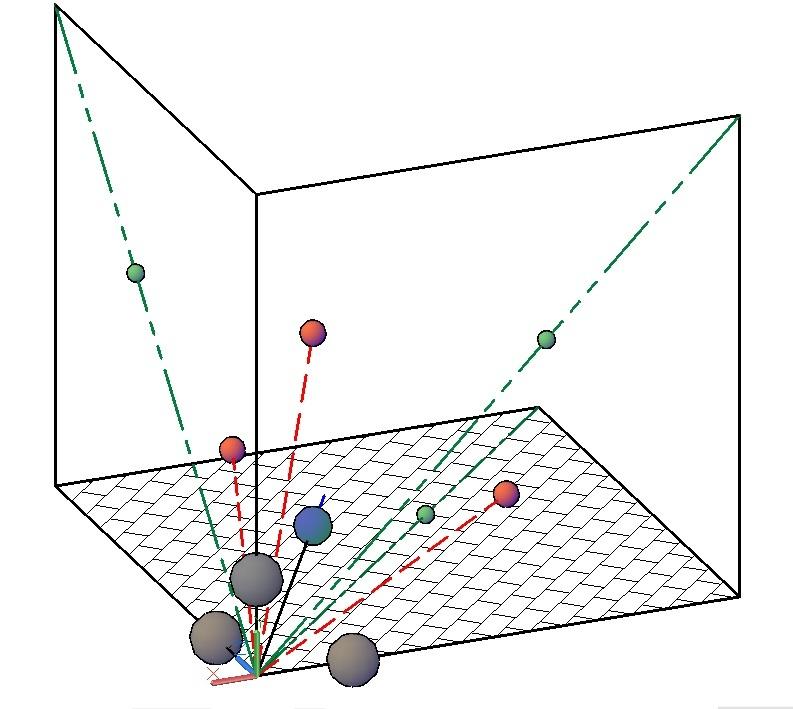
\includegraphics[width=0.3\textwidth]{3d4.jpg}
		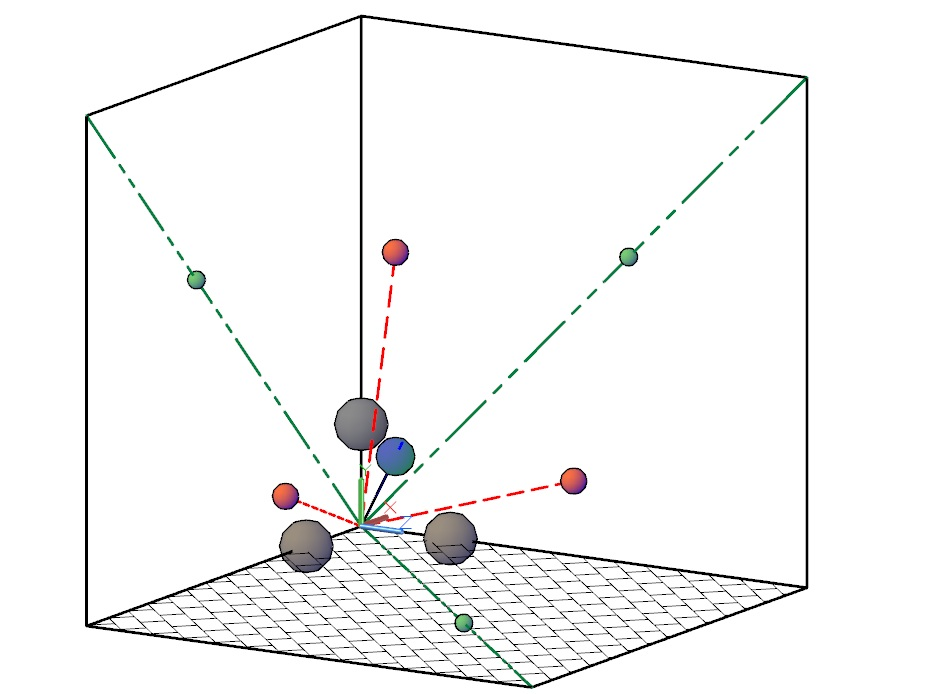
\includegraphics[width=0.3\textwidth]{3d3.jpg}
	\caption{distances and weights}
\end{figure}}
\end{frame}
%%%%%%%%%%%%%%%%%%%%%%%%%%%%%%%%
\begin{frame}
\frametitle{Moment constraint equations till 8th moment}
Only the even moments are shown that are to be satisfied. There are {\bf 11 non-zero moments for any dimension} in all
\begin{align*}
\uncover<2->{E[X_i^2]&=1 \quad &E[X_i^4]=3\\}
\uncover<3->{E[X_i^2X_j^2]&=1 \quad &E[X_i^6]=15\\}
\uncover<4->{E[X_i^4X_j^2]&=3 \quad &E[X_i^2X_j^2X_k^2]=1\\}
\uncover<5->{E[X_i^8]&=105 \quad &E[X_i^6X_j^2]=15\\}
\uncover<6->{E[X_i^4X_j^4]&=9 \quad &E[X_i^4X_j^2X_k^2]=3\\}
\uncover<7->{E[X_i^2X_j^2X_k^2X_l^2]&=1 \quad &\\}
\end{align*}\end{frame}
%%%%%%%%%%%%%%%%%%%%%%%%%%%%%%%%%%%%%%%%%%%%
\begin{frame}
\frametitle{Moment constraint equations till 8th moment for 4D system}
\small
\begin{align*}
2r_1^2w_1+16r_2^2w_2+12r_3^2w_3+16r_4^2w_4+24r_5^2w_5+48r_6^2w_6+16h^2r_6^2w_6=1\\
2r_1^4w_1+16r_2^4w_2+12r_3^4w_3+16r_4^4w_4+24r_5^4w_5+48r_6^4w_6+16h^4r_6^4w_6=3\\
16r_2^4w_2+4r_3^4w_3+16r_4^4w_4+16r_5^4w_5+32r_6^4w_6+32h^2r_6^4w_6=1\\
2r_1^6w_1+16r_2^6w_2+12r_3^6w_3+16r_4^6w_4+24r_5^6w_5+48r_6^6w_6+16h^6r_6^6w_6=15\\
16r_2^6w_2+4r_3^6w_3+16r_4^6w_4+16r_5^6w_5+32r_6^6w_6+16h^2r_6^6w_6+16h^4r_6^6w_6=3\\
16r_2^6w_2+16r_4^6w_4+8r_5^6w_5+16r_6^6w_6+48h^2r_6^6w_6=1\\
2r_1^8w_1+16r_2^8w_2+12r_3^8w_3+16r_4^8w_4+24r_5^8w_5+48r_6^8w_6+16h^8r_6^8w_6=105\\
16r_2^8w_2+4r_3^8w_3+16r_4^8w_4+16r_5^8w_5+32r_6^8w_6+16h^2r_6^8w_6+16h^6r_6^8w_6=15\\
16r_2^8w_2+4r_3^8w_3+16r_4^8w_4+16r_5^8w_5+32r_6^8w_6+32h^4r_6^8w_6=9\\
16r_2^8w_2+16r_4^8w_4+8r_5^8w_5+16r_6^8w_6+32h^2r_6^8w_6+16h^4r_6^8w_6=3\\
16r_2^8w_2+16r_4^8w_4+64h^2r_6^8w_6=1
\end{align*}     
\end{frame}
%%%%%%%%%%%%%%%%%%%%%%%%%%%%%%%%%%%%%%%%%%%
\begin{frame}
\frametitle{Moment constraint equations till 8th moment for 5D system}
\small
\begin{align*}
2r_1^2w_1+32r_2^2w_2+16r_3^2w_3+32r_4^2w_4+48r_5^2w_5+128r_6^2w_6+32h^2r_6^2w_6&=1\\
2r_1^4w_1+32r_2^4w_2+16r_3^4w_3+32r_4^4w_4+48r_5^4w_5+128r_6^4w_6+32h^4r_6^4w_6&=3\\
32r_2^4w_2+4r_3^4w_3+32r_4^4w_4+24r_5^4w_5+96r_6^4w_6+64h^2r_6^4w_6&=1\\
2r_1^6w_1+32r_2^6w_2+16r_3^6w_3+32r_4^6w_4+48r_5^6w_5+128r_6^6w_6+32h^6r_6^6w_6&=15\\
32r_2^6w_2+4r_3^6w_3+32r_4^6w_4+24r_5^6w_5+96r_6^6w_6+32h^2r_6^6w_6+32h^4r_6^6w_6&=3\\
32r_2^6w_2+32r_4^6w_4+8r_5^6w_5+64r_6^6w_6+96h^2r_6^6w_6&=1\\
2r_1^8w_1+32r_2^8w_2+16r_3^8w_3+32r_4^8w_4+48r_5^8w_5+128r_6^8w_6+32h^8r_6^8w_6&=105\\
32r_2^8w_2+4r_3^8w_3+32r_4^8w_4+24r_5^8w_5+96r_6^8w_6+32h^2r_6^8w_6+32h^6r_6^8w_6&=15\\
32r_2^8w_2+4r_3^8w_3+32r_4^8w_4+24r_5^8w_5+96r_6^8w_6+64h^4r_6^8w_6&=9\\
32r_2^8w_2+32r_4^8w_4+8r_5^8w_5+64r_6^8w_6+64h^2r_6^8w_6+32h^4r_6^8w_6&=3\\
32r_2^8w_2+32r_4^8w_4+32r_6^8w_6+128h^2r_6^8w_6&=1\\
\end{align*}
\end{frame}
%%%%%%%%%%%%%%%%%%%%%%%%%%%%%%%%
\begin{frame}
\frametitle{Solution for 5D system}
\small
\begin{align}
h&=3 \nonumber \\
r_5&=2\nonumber\\
r_1&=2.3143708172807447\nonumber\\
r_2&=0.8390942773980102\nonumber\\
r_3&=1.8307521253266494\nonumber\\
r_4&=1.3970397430644959\nonumber\\
r_6&=1.1134786327367021\nonumber\\
w_1 &= 0.010529034221546607\nonumber\\
w_2 &= 0.015144019639537572\nonumber\\
w_3 &= 0.0052828996967816825\nonumber\\
w_4&=0.0010671298950159158\nonumber\\
w_5&=0.0006510416666666666\nonumber\\
w_6 &= 0.00013776017592074394 
\end{align}
\end{frame}
%%%%%%%%%%%%%%%%%%%%%%%%%%%%%%%
\begin{frame}
\frametitle{}
{\bf Results of integration compared to Gauss Hermite integration for 5D system}\newline
For a N-D system the total number of points required to capture the 8th moment  by this scheme are \newline $1+2N^2+\frac{4N(N-1)(N-2)}{3}+(N+2)2^N$.\newline
 The covariance of the gaussian Kernel
\begin{align}
P=1000I_{5x5}
\end{align}
\begin{align}
X&=[x_1,x_2,x_3,x_4,x_5]\\
F(X)&=x_1^8+x_2^8+x_3^6+x_4^6+x_1^4x_5^4+x_2^4x_3^4+x_4^2+x_1^2x_2^2x_3^2x_4^2+\nonumber \\
&+x_1^3x_3+x_1^4x_2^2x_5^2+x_3^4x_2^2+x_1^2x_3^4+x_1^3x_3+x_2^3x_3+x_3^3x_2
\end{align}
Evaluating the integral
\begin{equation}
f=\int{F(X)N(X,0|P)}dX
\end{equation}
\end{frame}
%%%%%%%%%%%%%%%%%%%%%%%%%%
\begin{frame}
\begin{center}
\tiny
  \begin{tabular}{ | l | l | l | l | l | l | }
    \hline
       No. of pts 					& $2^5=$ 32 				& $3^5=$ 243 			   & $4^5=$ 1024			   & $5^5=$ 3125  	    &  $15^5=$759375(Truth)                \\ \hline 
       GH          					& 6.0962801e+012 		& 7.6616634e+013     & 1.84964e+014      	 & 2.329646e+014  		  &   2.3296463e+014           \\ \hline
    \% error            	  & 97.38317      		&  67.11233  	    	 & 20.6039857          & 5.184531e-011       &   0                     \\ 
      \hline 
  \end{tabular}
\end{center} 
\uncover<2->{
\begin{center}
  \begin{tabular}{ | l | l | l | l | l | }
    \hline
                  					&   No. of pts			& Integration result 			    & \% error wrt Truth			 \\ \hline 
      NM          					&   355       		  & 2.3296463e+014              & 5.1509964e-011   \\
      \hline
  \end{tabular}
\end{center}}
\end{frame}
%%%%%%%%%%%%%%%%%%%%%%%%%%%%%%%%%%%
\begin{frame}
\frametitle{Results for Non- Polynomial Nonlinearity}
{\bf Polar to Cartesian coordinates transformation}
\begin{itemize}[<+->]
\item A radar has error in its radial and angular measurements
\item We would like to see how this error is transformed into cartesian coordinates
\item We would like to compute the expected value in the cartesian coordinates
\end{itemize}
\uncover<5->{In effect we are trying to evaluate the integral
\begin{align*}
E[(x,y)^T]&=E[(rcos(\theta),rsin(\theta))^T]\\
&=\int{\int{(rcos(\theta),rsin(\theta))^T N((r,\theta),(\mu_r,\mu_{\theta}|P))}}drd\theta
\end{align*}}
\end{frame}
%%%%%%%%%%%%%%%%%%%%%%
\begin{frame}
   \begin{figure}[thpb]
      \centering
      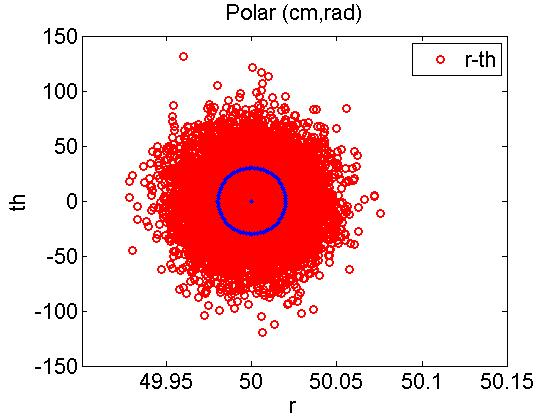
\includegraphics[width=1\textwidth]{polar}
      \caption{2D and 3D Cubature points to satisfy 6th order moments}
      \label{fig:23d4m1}
   \end{figure} 
\end{frame}
%%%%%%%%%%%%%%%%%%%%%%
\begin{frame}
   \begin{figure}[thpb]
      \centering
      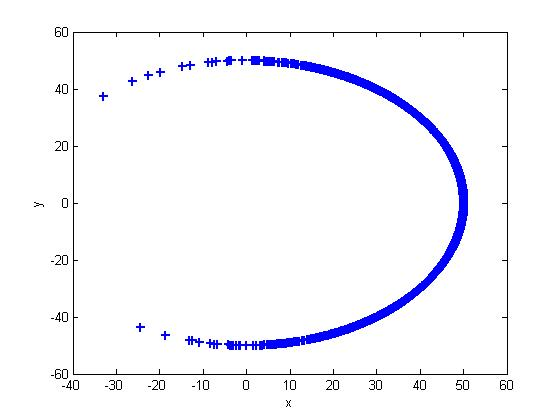
\includegraphics[width=1\textwidth]{polartocart2}
      \caption{2D and 3D Cubature points to satisfy 6th order moments}
      \label{fig:23d4m1}
   \end{figure} 
\end{frame}
%%%%%%%%%%%%%%%%%%%%%%%
\begin{frame}   
   \begin{figure}[thpb]
      \centering
      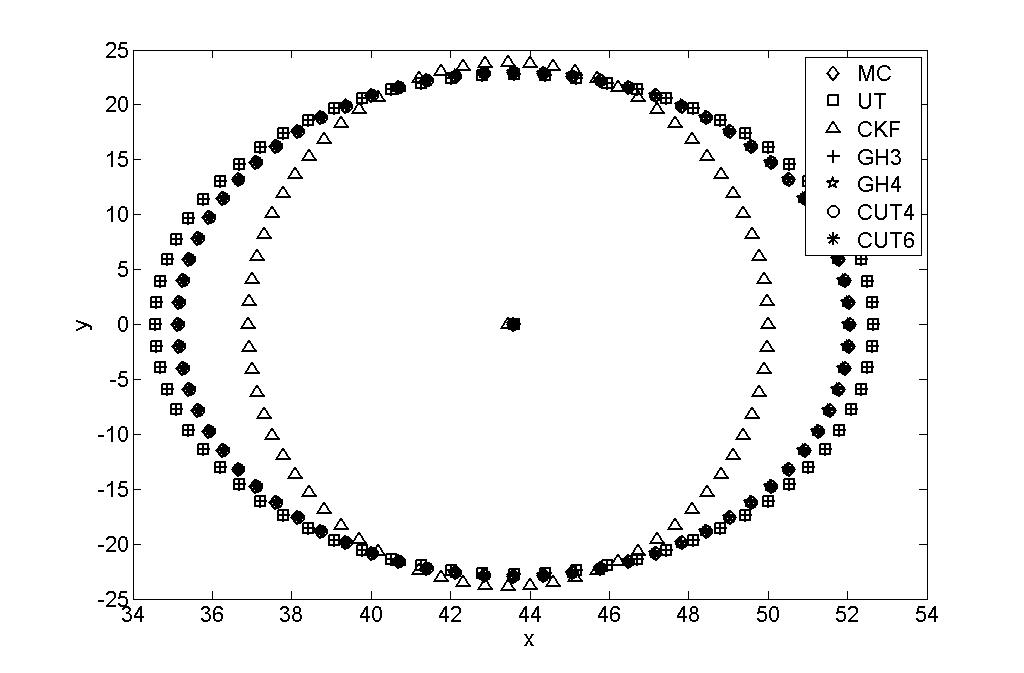
\includegraphics[width=1\textwidth]{polartocart}
      \caption{2D and 3D Cubature points to satisfy 6th order moments}
      \label{fig:23d4m1}
   \end{figure} 
\end{frame}
%%%%%%%%%%%%%%%%%%%%%
\begin{frame}
\frametitle{Expected value of Normal PDF}
{\bf Normal Distribution}
The integral being evaluated is 
\begin{equation*}
E[N(x,\mu|P)]=\int{N(x,\mu|P)N(x,\mu|P)}dx
\end{equation*}
The parameters used are
\begin{align*}
\mu&=0\\
P&=I
\end{align*}
\end{frame}
%%%%%%%%%%%%%%%%%%%%%%%%%%%
\begin{frame}
\frametitle{True value of Integral}
   \begin{figure}[thpb]
      \centering
      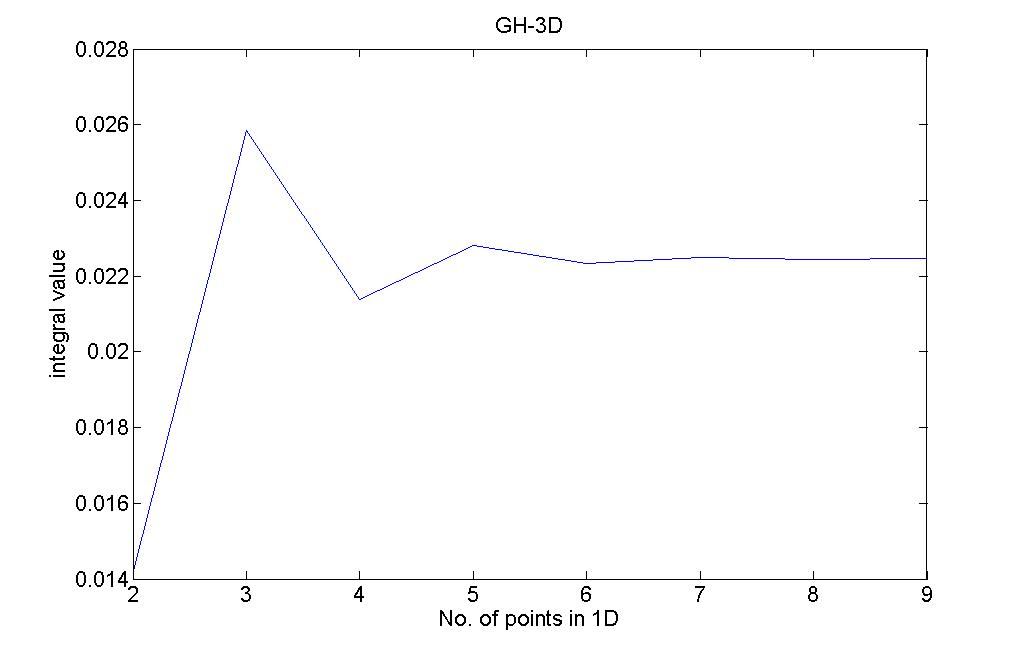
\includegraphics[width=0.5\textwidth]{3dGH_for_gauss_sqr.jpg}
      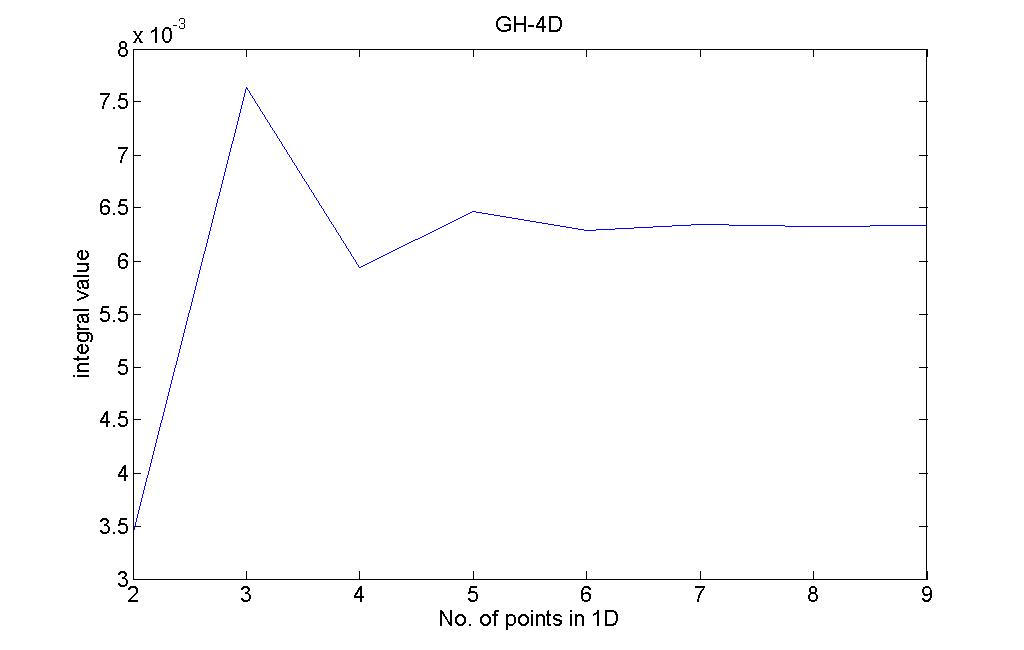
\includegraphics[width=0.5\textwidth]{4dGH_for_gauss_sqr.jpg}
      \label{fig:23d4m1}
   \end{figure} 

   \begin{figure}[thpb]
      \centering
      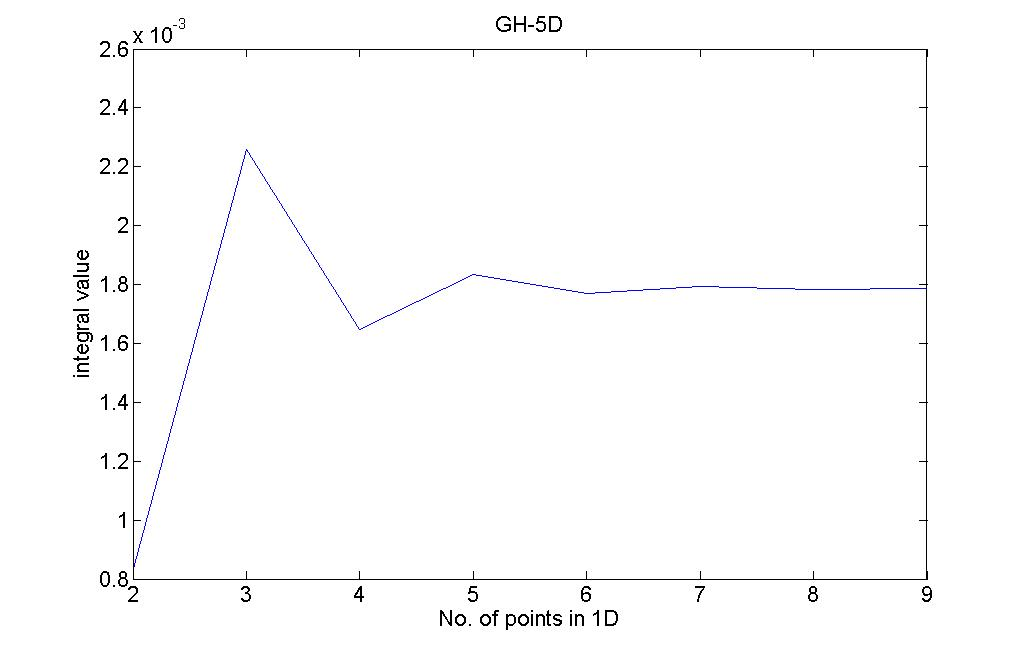
\includegraphics[width=0.5\textwidth]{5dGH_for_gauss_sqr.jpg}
      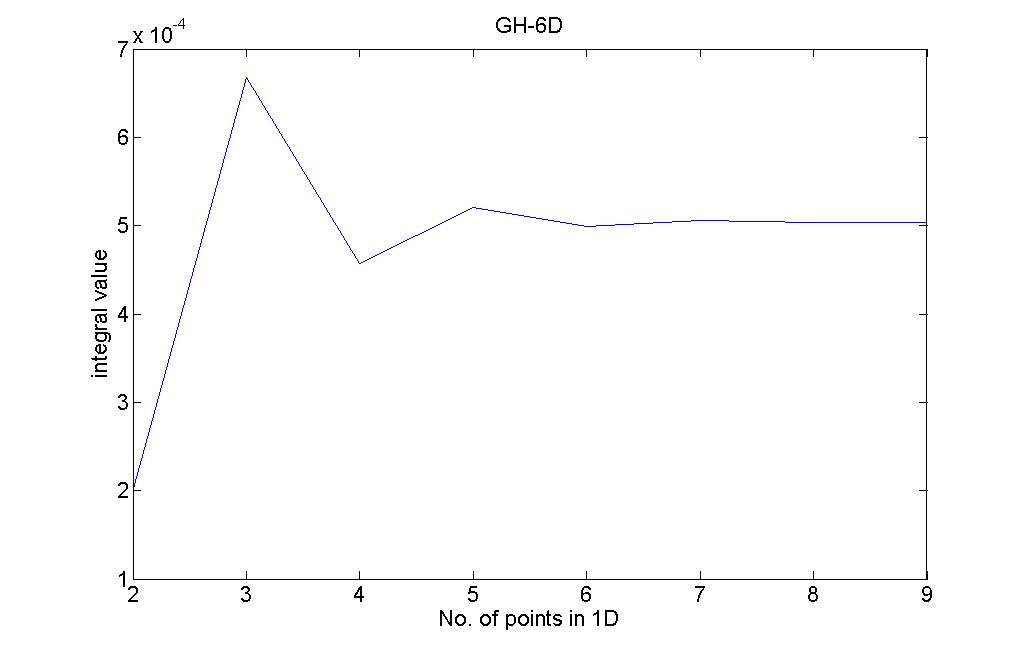
\includegraphics[width=0.5\textwidth]{6dGH_for_gauss_sqr.jpg}
   \end{figure} 
\end{frame}
%%%%%%%%%%%%%%%%%%%%%
\begin{frame}
\begin{table}
\caption{Results of the integration interms of \% rel. error }
\label{optsoln12}
\begin{center}

\begin{tabular}{|c||c|c|c|c|c|}
\hline
Dimension & CKF & UT & CUT4 & CUT6 & CUT8 \\
\hline
$3$ & $36.902 $  &  $36.902$ & $27.042$ & $13.273$ & $1.5688$  \\
\hline
$4$ & $45.880 $  &  $45.880 $ &  $46.571$ &  $23.276 $ & $2.0279$\\
\hline
$5$ & $53.581 $  &  $53.581 $ &  $73.768$ & $28.056 $ & $6.8219$\\
\hline
$6$ & $60.186$  &  $60.186 $ & $110.90$ & $13.393$ & $15.793$\\
\hline
\end{tabular}
\end{center}
\end{table}

\begin{table}
\caption{Number of points in each method }
\label{optsoln12}
\begin{center}
\small
\begin{tabular}{|c||c|c|c|c|c|c|c|c|}
\hline
Dim & GH-5     &  GH-6     &  GH-7      & CKF   & UT    & CUT4  & CUT6  & CUT8 \\
\hline
$3$       & $125 $   &  $216$    &  $343$    & $6$   & $7$   & $15$   & $27$   & $59$\\
\hline
$4$       & $625 $  &  $1296$   &  $2401$   & $8$   & $9$   & $25$   & $49$   & $161$\\
\hline
$5$       & $3125  $  &  $7776 $ &  $ 16807$   & $10$  & $11$  & $43$   & $83$   & $355$\\
\hline
$6$       & $15625$   &  $46656$  &  $117649$  & $12$  & $13$  & $77$   & $137$   & $745$\\
\hline
\end{tabular}
\end{center}
\end{table}
\end{frame}
%%%%%%%%%%%%%%%%%%%%%
\begin{frame}
\frametitle{Expected value of Exponential Function}
{\bf Normal Distribution}
The integral being evaluated is 
\begin{equation*}
E[N(x,\mu|P)]=\int{exp(-\sum_{i=1}^N{x_i})N(x,\mu|P)}dx
\end{equation*}
 The parameters used are
\begin{align*}
\mu&=0\\
P&=I
\end{align*}
\end{frame}
%%%%%%%%%%%%%%%%%%%%%
%%%%%%%%%%%%%%%%%%%%%%%%%%%
\begin{frame}
\frametitle{True value of Integral}
   \begin{figure}[thpb]
      \centering
      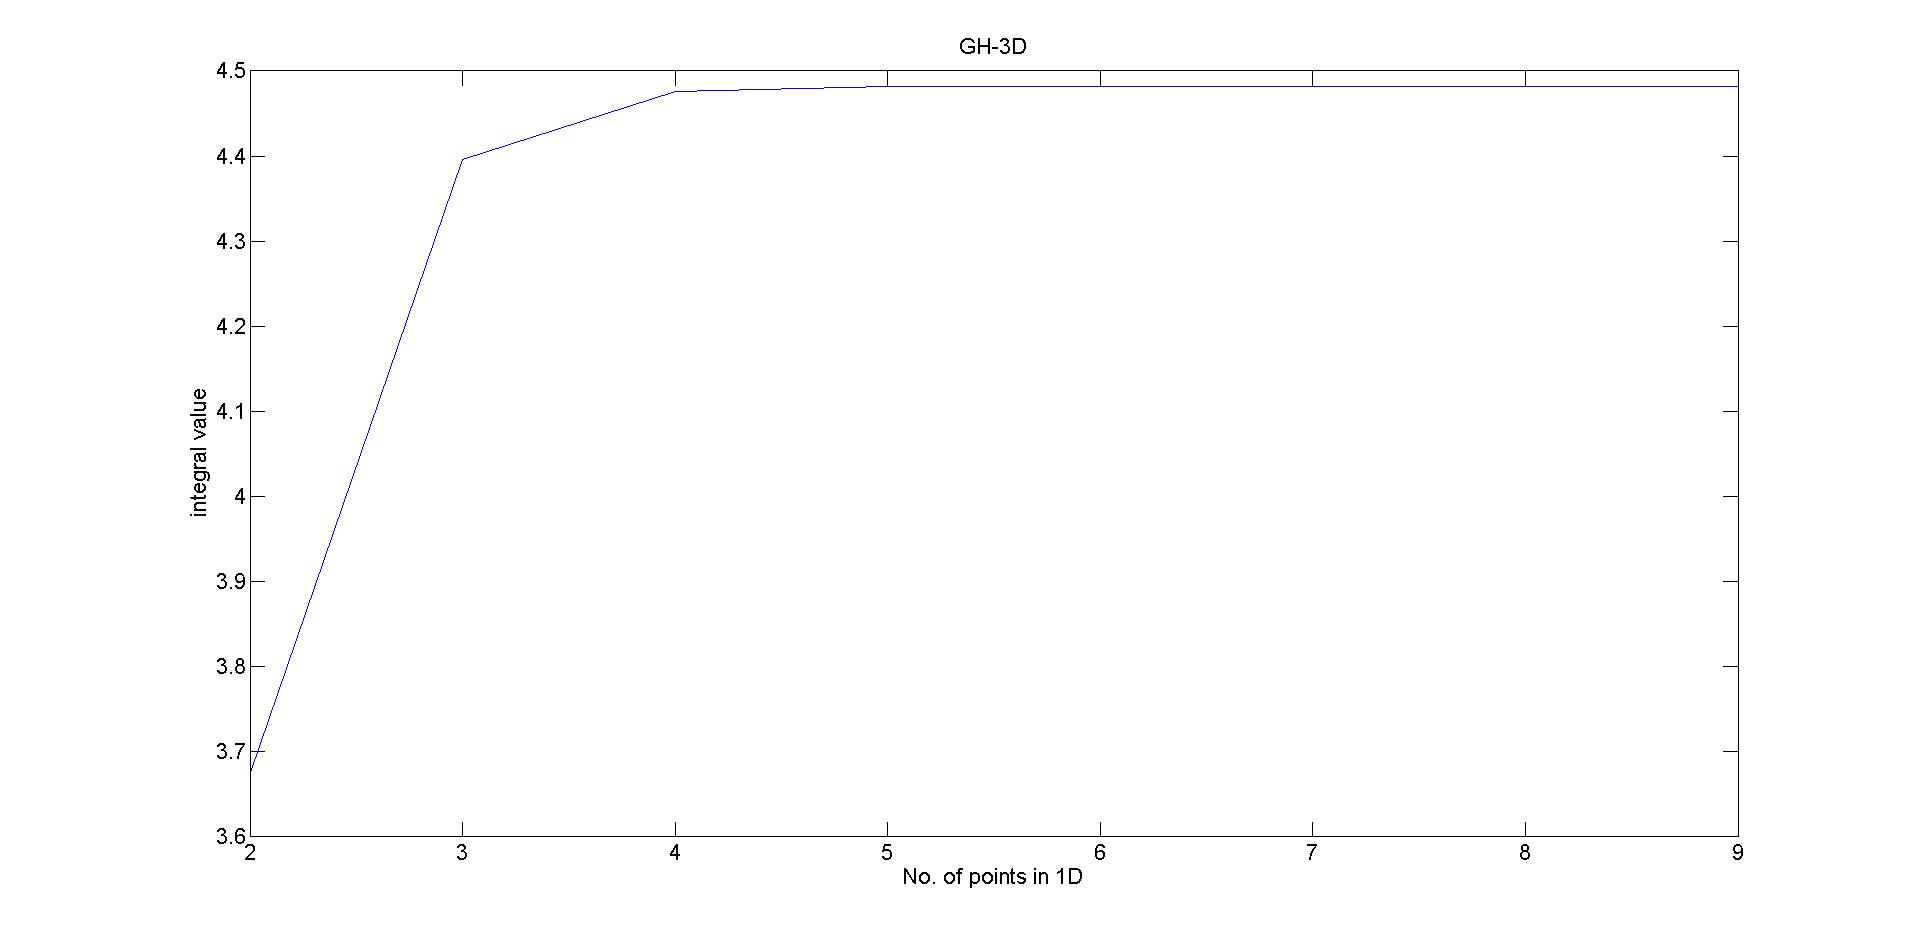
\includegraphics[width=0.5\textwidth]{3dGH_for_exp.jpg}
      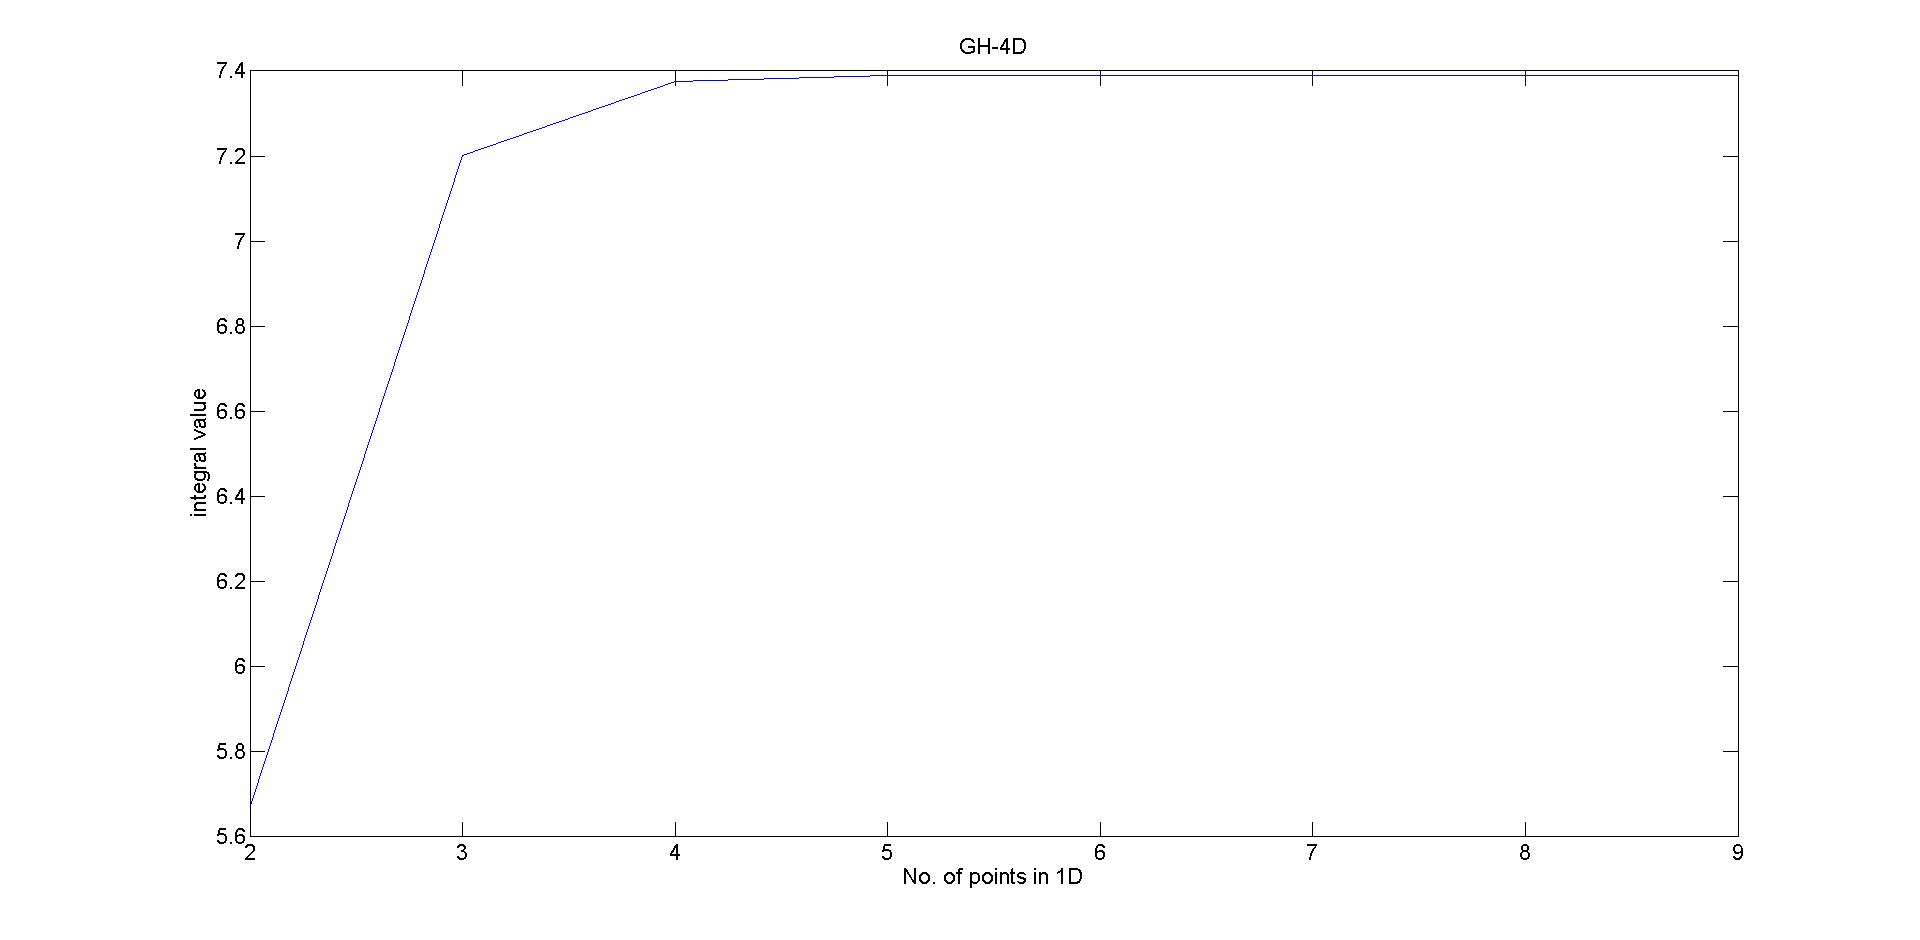
\includegraphics[width=0.5\textwidth]{4dGH_for_exp.jpg}
      \label{fig:23d4m1}
   \end{figure} 

   \begin{figure}[thpb]
      \centering
      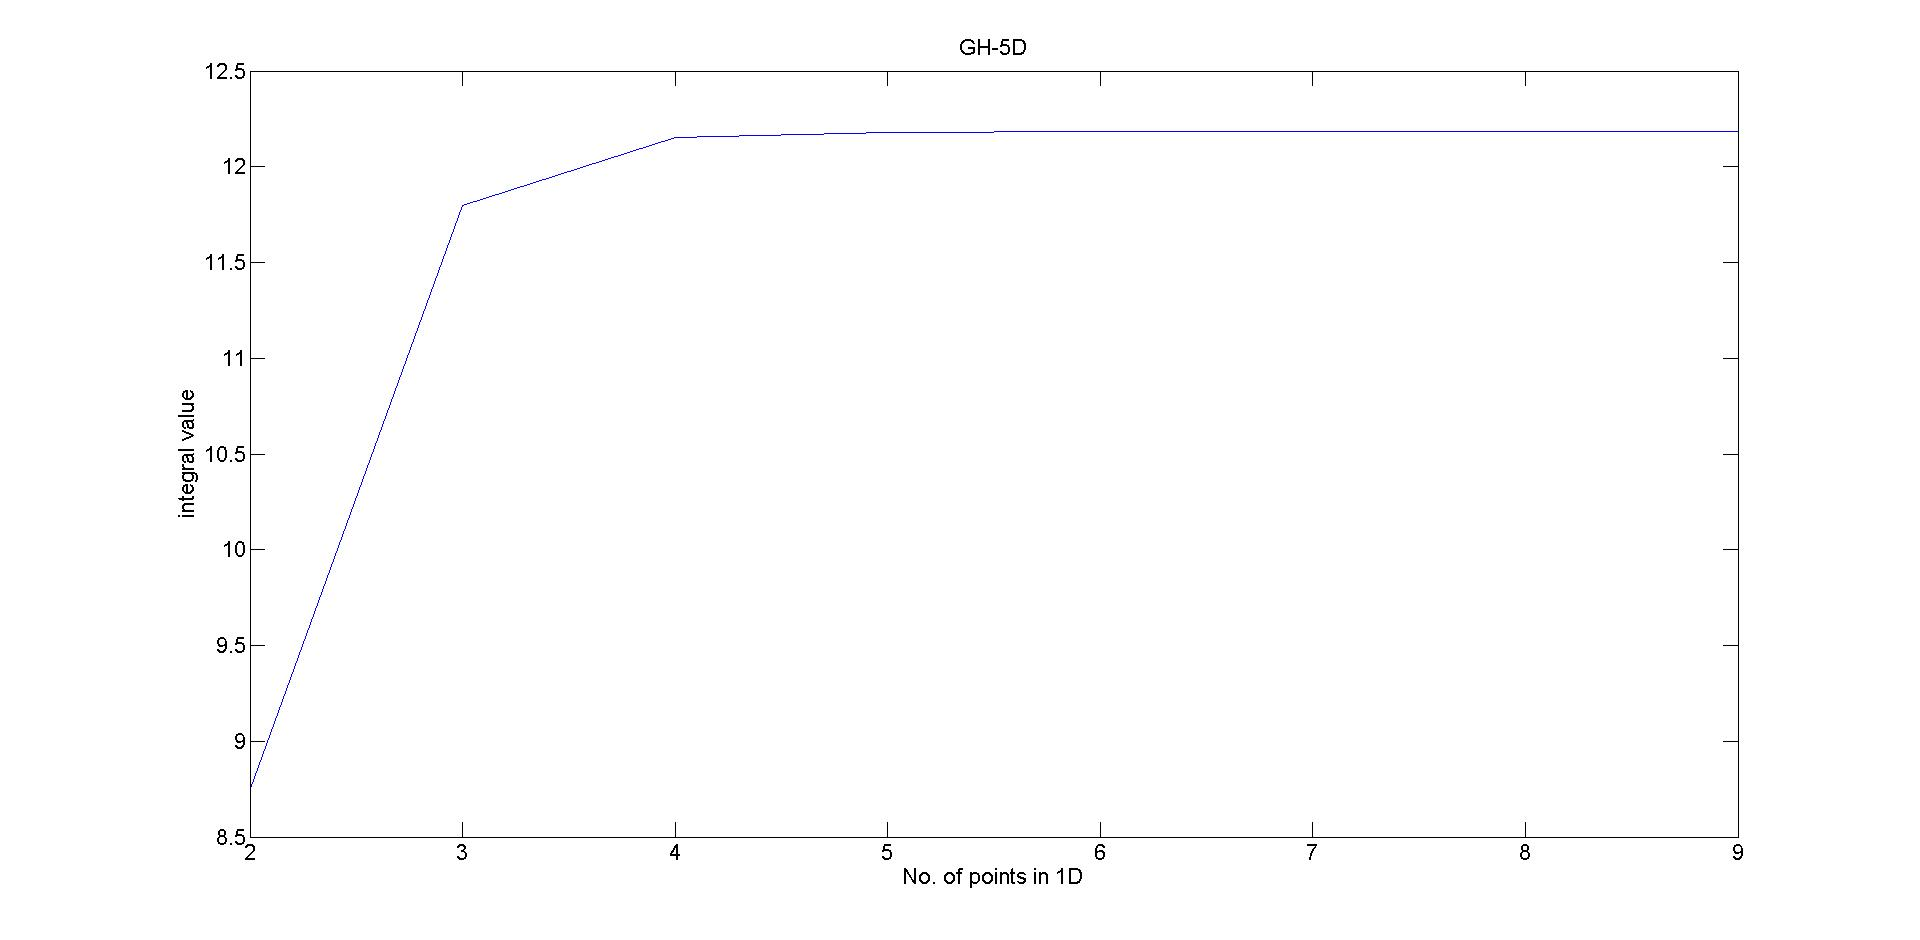
\includegraphics[width=0.5\textwidth]{5dGH_for_exp.jpg}
      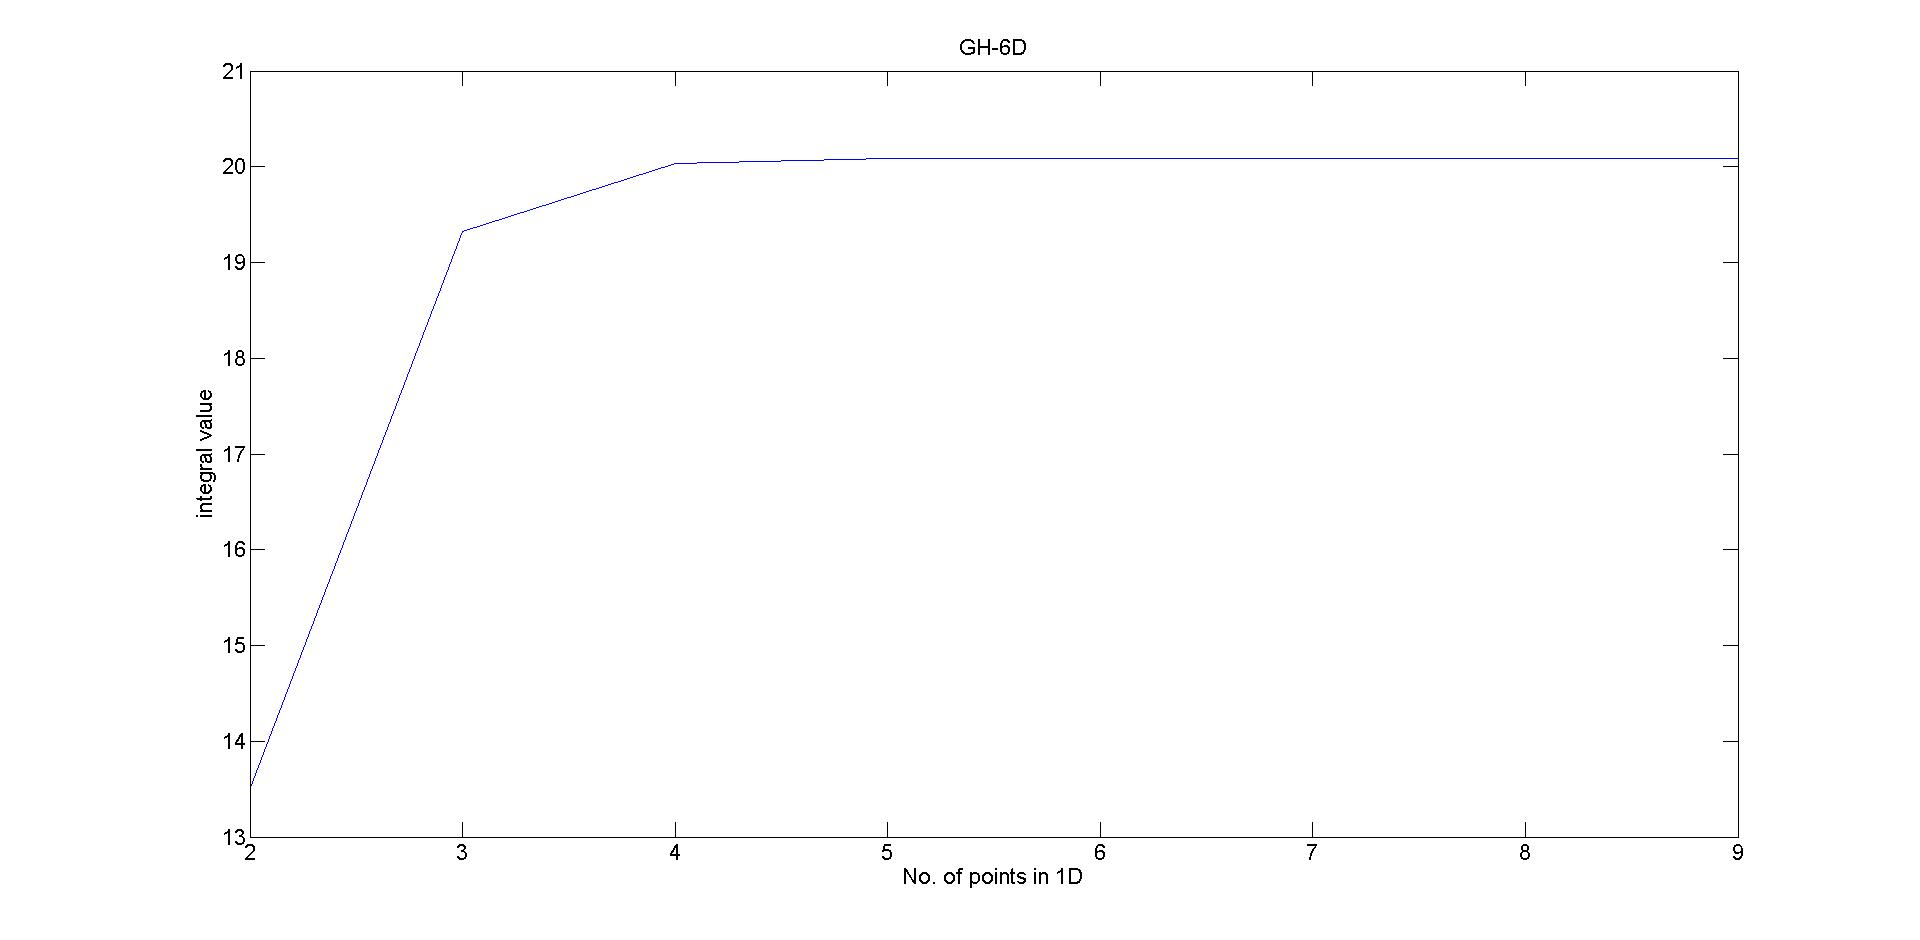
\includegraphics[width=0.5\textwidth]{6dGH_for_exp.jpg}
   \end{figure} 
\end{frame}
%%%%%%%%%
\begin{frame}
\begin{table}
\caption{Results of the integration interms of \% rel. error }
\label{optsoln12}
\begin{center}

\begin{tabular}{|c||c|c|c|c|c|}
\hline
Dimension & CKF & UT & CUT4 & CUT6 & CUT8 \\
\hline
$3$ & $34.9670 $  &  $34.9670$ & $5.6510$ & $1.5589$ & $0.0813$  \\
\hline
$4$ & $49.0842 $  &  $49.0842 $ &  $7.7049$ &  $2.0998 $ & $0.6467$\\
\hline
$5$ & $61.1601 $  &  $61.1601 $ &  $9.7754$ & $7.0631 $ & $1.4656$\\
\hline
$6$ & $70.9523$  &  $70.9523 $ & $12.0018$ & $11.6941$ & $1.2176$\\
\hline
\end{tabular}
\end{center}
\end{table}

\begin{table}
\caption{Number of points in each method }
\label{optsoln12}
\begin{center}
\small
\begin{tabular}{|c||c|c|c|c|c|c|c|c|}
\hline
Dim    &  GH-4  & GH-5     &  GH-6         & CKF   & UT    & CUT4  & CUT6  & CUT8 \\
\hline
$3$    & $64$  & $125 $   &  $216$    &      $6$   & $7$   & $15$   & $27$   & $59$\\
\hline
$4$    & $256$  & $625 $  &  $1296$   &   $8$   & $9$   & $25$   & $49$   & $161$\\
\hline
$5$   &  $1024$  & $3125 $  &  $7776 $ &   $10$  & $11$  & $43$   & $83$   & $355$\\
\hline
$6$    & $4096$  & $15625$   &  $46656$  &   $12$  & $13$  & $77$   & $137$   & $745$\\
\hline
\end{tabular}
\end{center}
\end{table}
\end{frame}
%%%%%%%%%%%%%%%%%%%%%
\begin{comment}
\frametitle{Expected value of Delta 'like' Function}
{\bf Normal Distribution}
The integral being evaluated is 
\begin{equation*}
E[(\sqrt{1+x^Tx})^p]=\int{(\sqrt{1+x^Tx})^pN(x,\mu|P)}dx
\end{equation*}
\end{comment}

%%%%%%%%%%%%%%%%%%%%%
\begin{frame}
\frametitle{Discussion}
\begin{itemize}[<+->]
\item Is there a better way to solve the fully nonlinear system of moment equations. 
\item How to find the minimal number of cubature points -or- to be optimistic how to prove that the cubature points by this method is minimal.
\item Is it really advantageous to develop higher order methods from a filtering point of view. If the first approximation is dominantly wrong does it help in using higher order cubature points

\end{itemize}
\end{frame}
%%%%%%%%%%%%%%%%%%%%%
\begin{frame}
\frametitle{Discussion}
\begin{itemize}[<+->]
\item How to identify the non-polynomial type of functions that can be integrated by these methods accurately .- How do we develop Error estimates. For example for 1D Gauss Hermite quadrature the error estimate is $E=\frac{n!\sqrt{\pi}}{2^n(2n)!}f^{2n}(\xi)$ 
\item How do we generalize this method or how do we find a mathematically rigorous theory/algorithm to generate cubature points for any moment and any dimension.
\item Can we find the cubature points for any other PDF in the same manner.
\end{itemize}
\end{frame}
%%%%%%%%%%%%%%%%%%%%%
%%%%%%%%%%%%%%%%%%%%%
\end{document}